\chapter{Results and Comparisons} 
\label{ch:results} 

\section{Test Case 1}

\begin{figure}
  \centering
  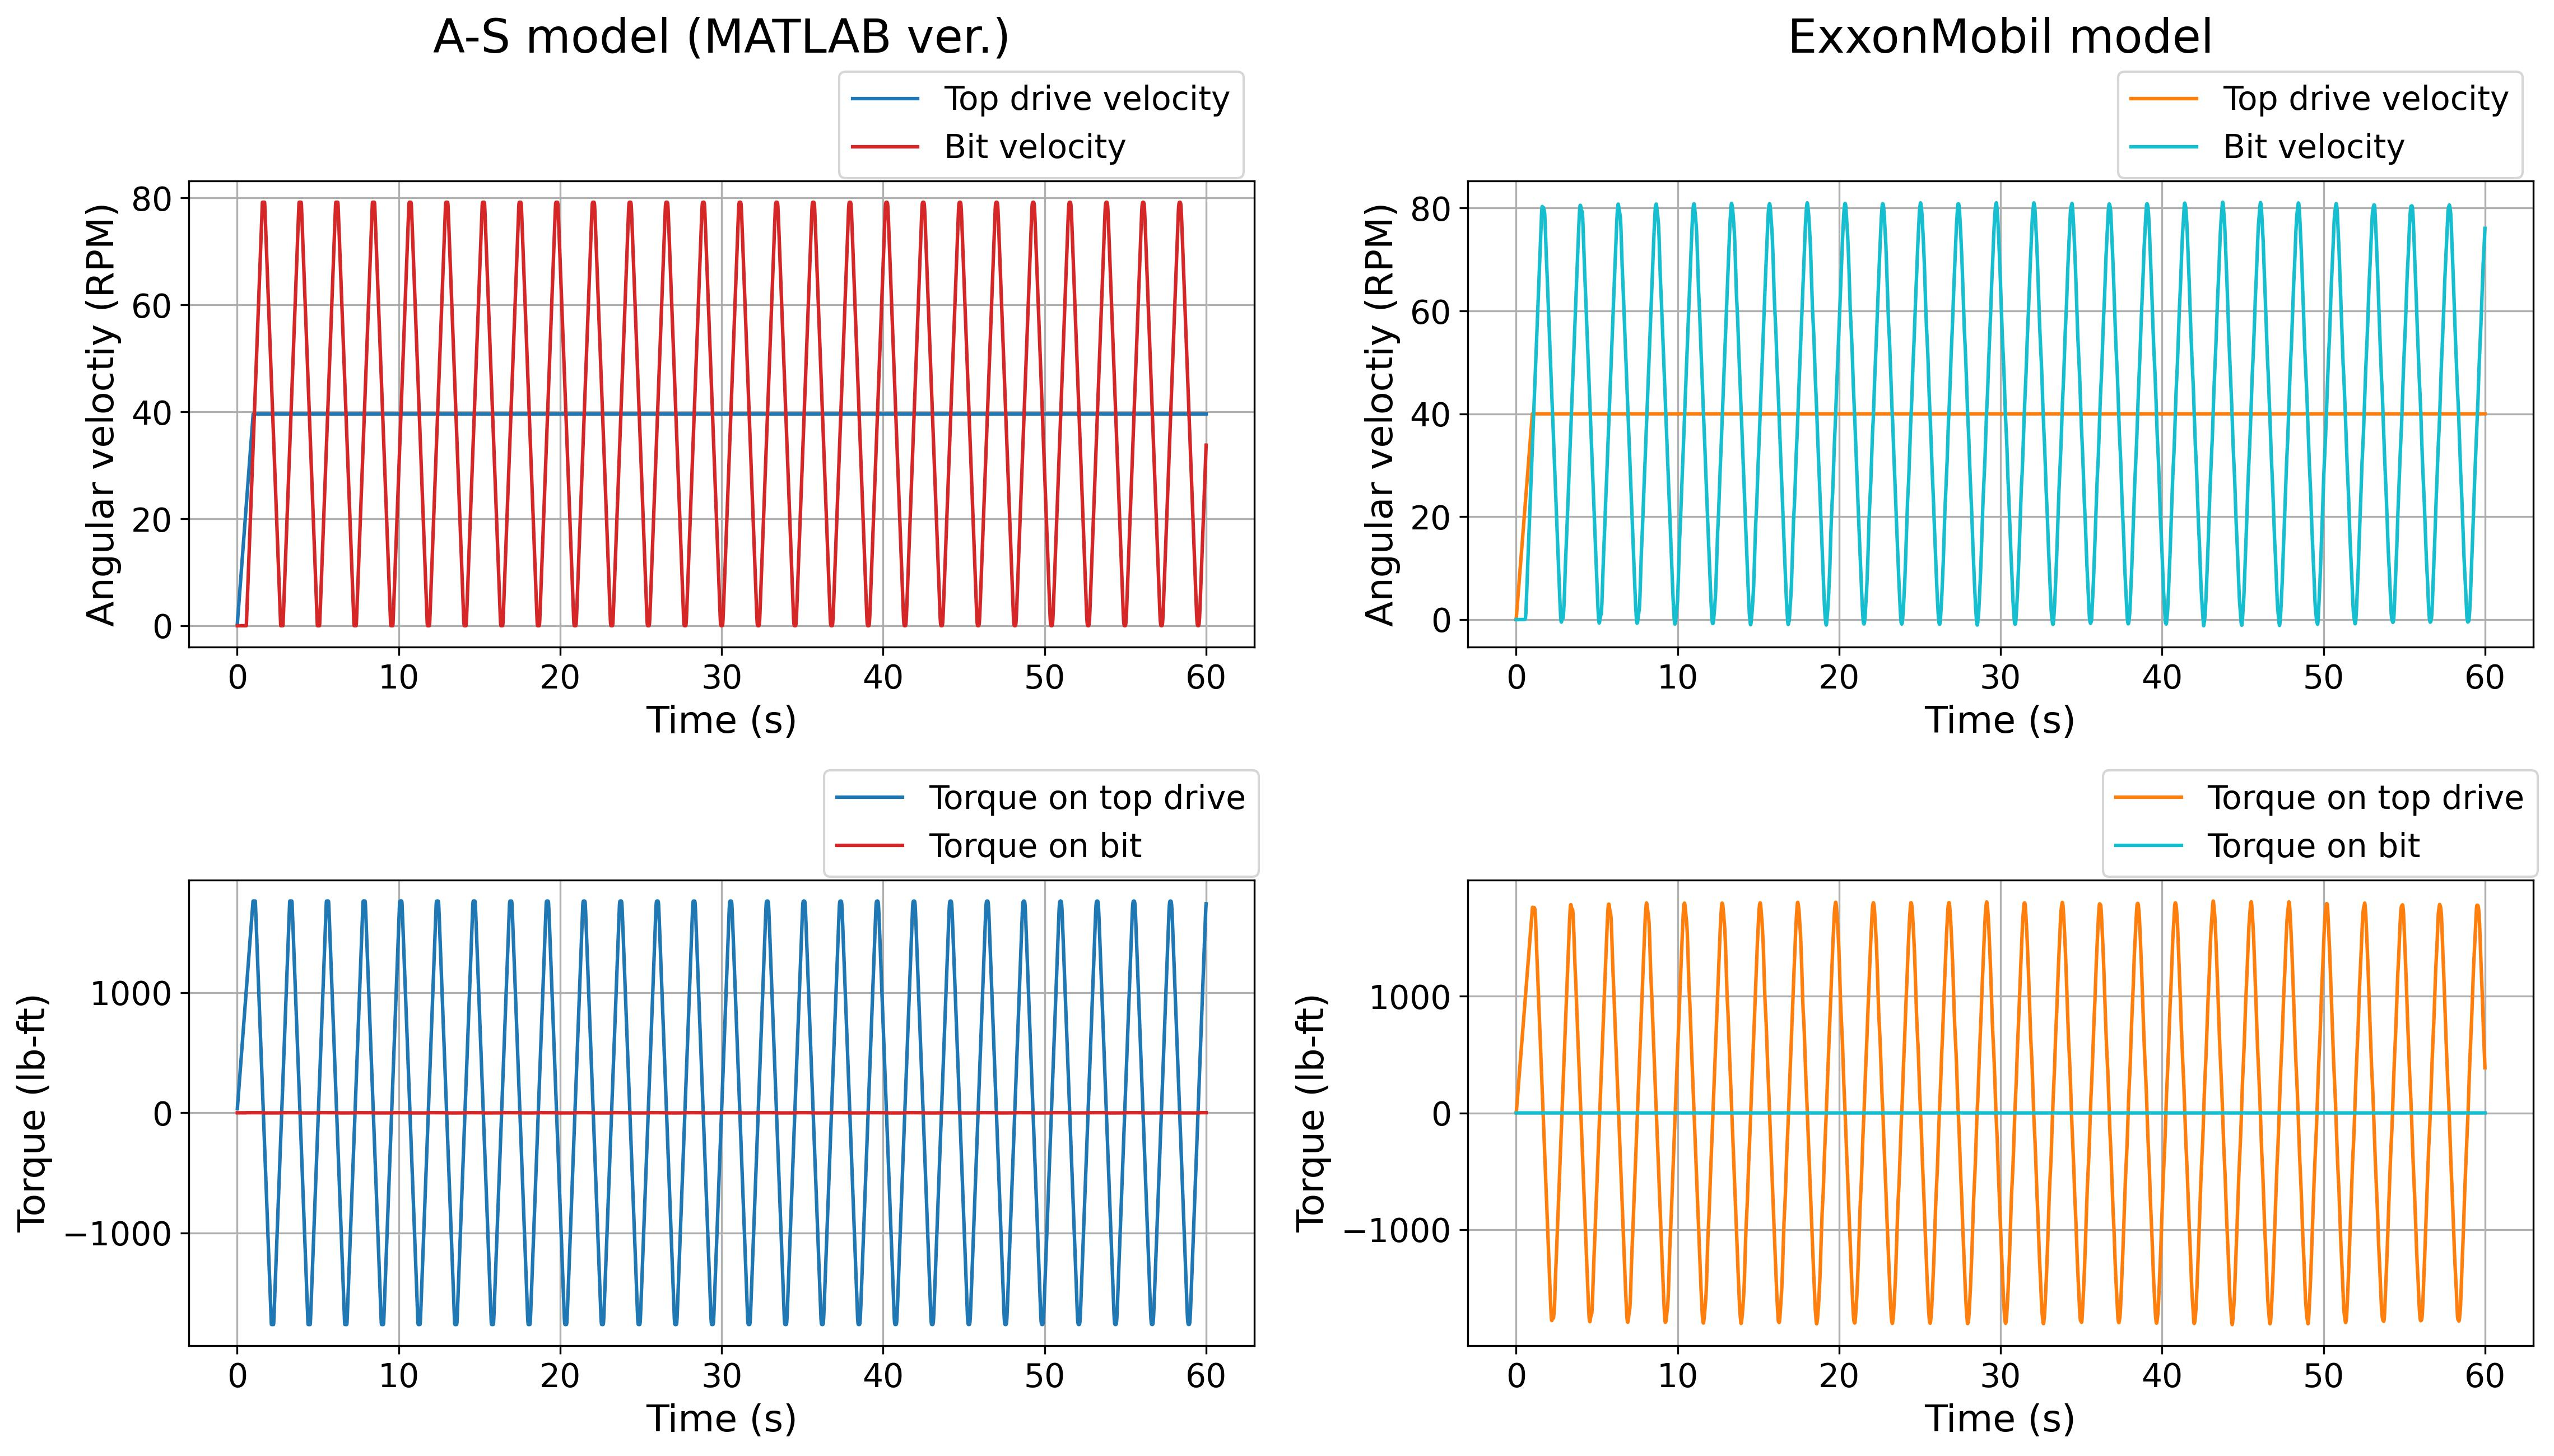
\includegraphics[width=6.5in]{output_figureTestCase1}
  \caption{}\label{figure_testcase1}
\end{figure}
\begin{figure}
  \centering
  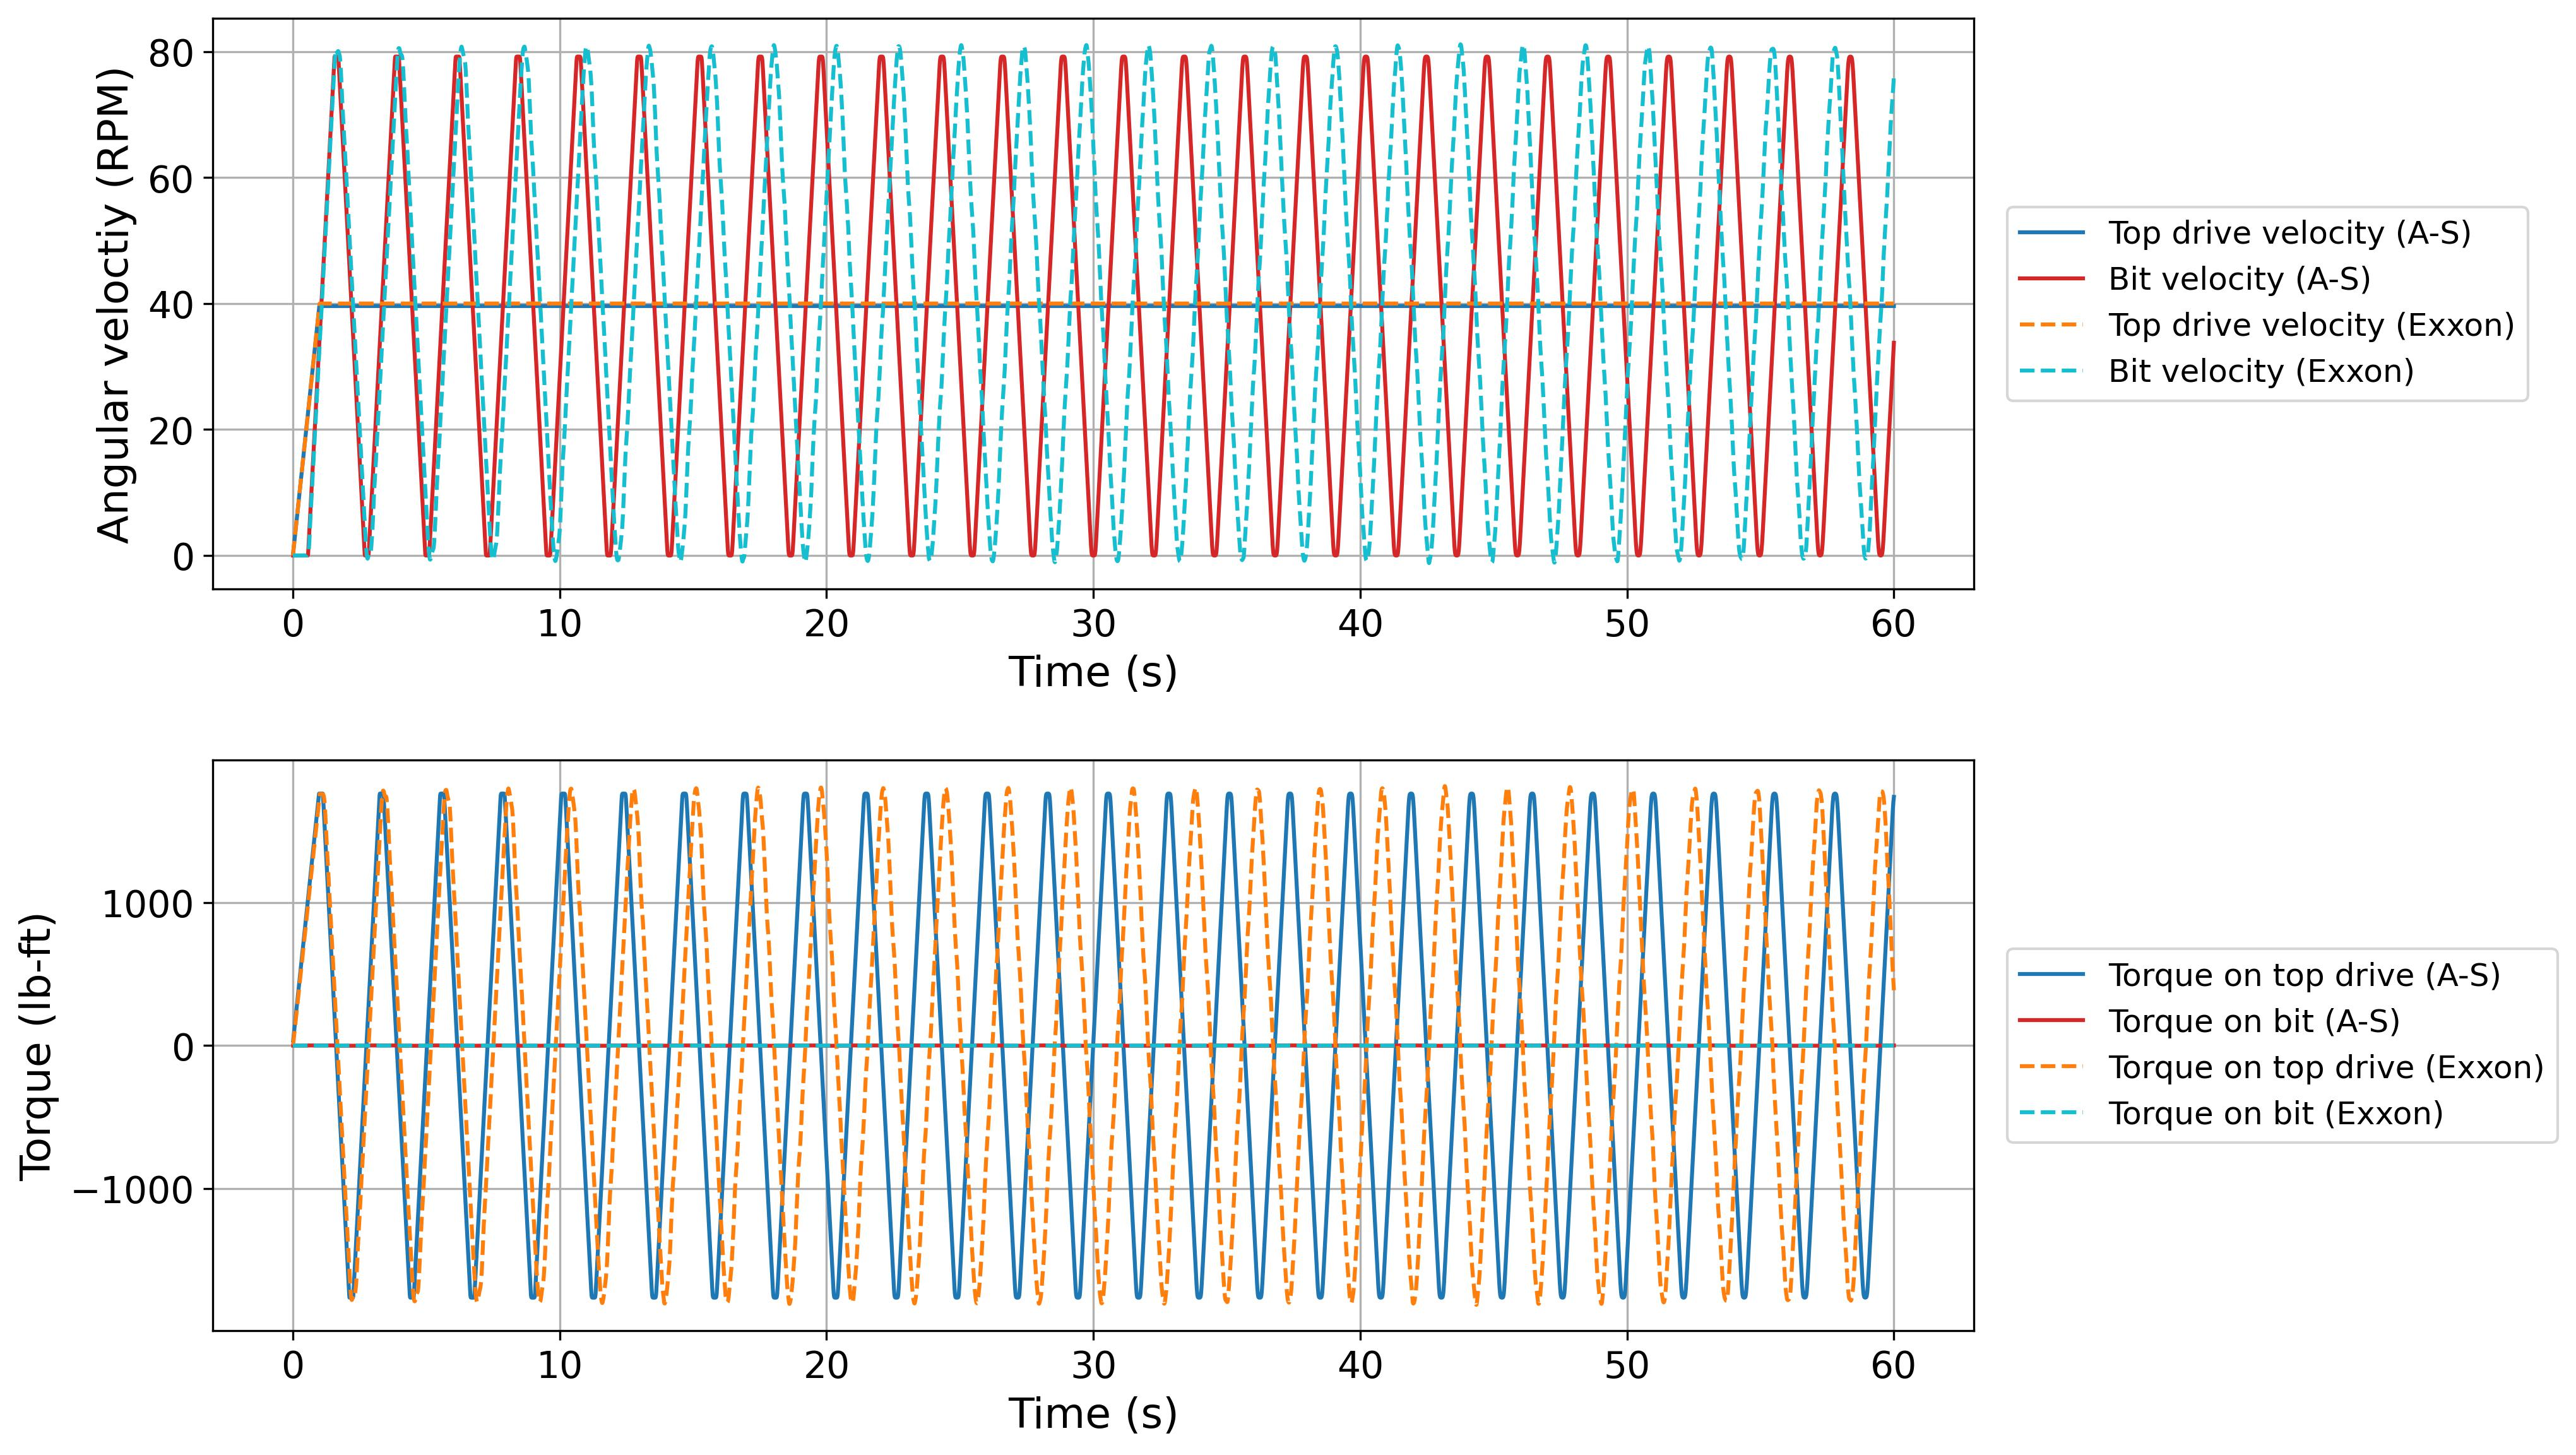
\includegraphics[width=6.5in]{overlapped_figureTestCase1}
  \caption{}\label{figure_testcase1_overlapped}
\end{figure}

\section{Test Case 2}

\begin{figure}
  \centering
  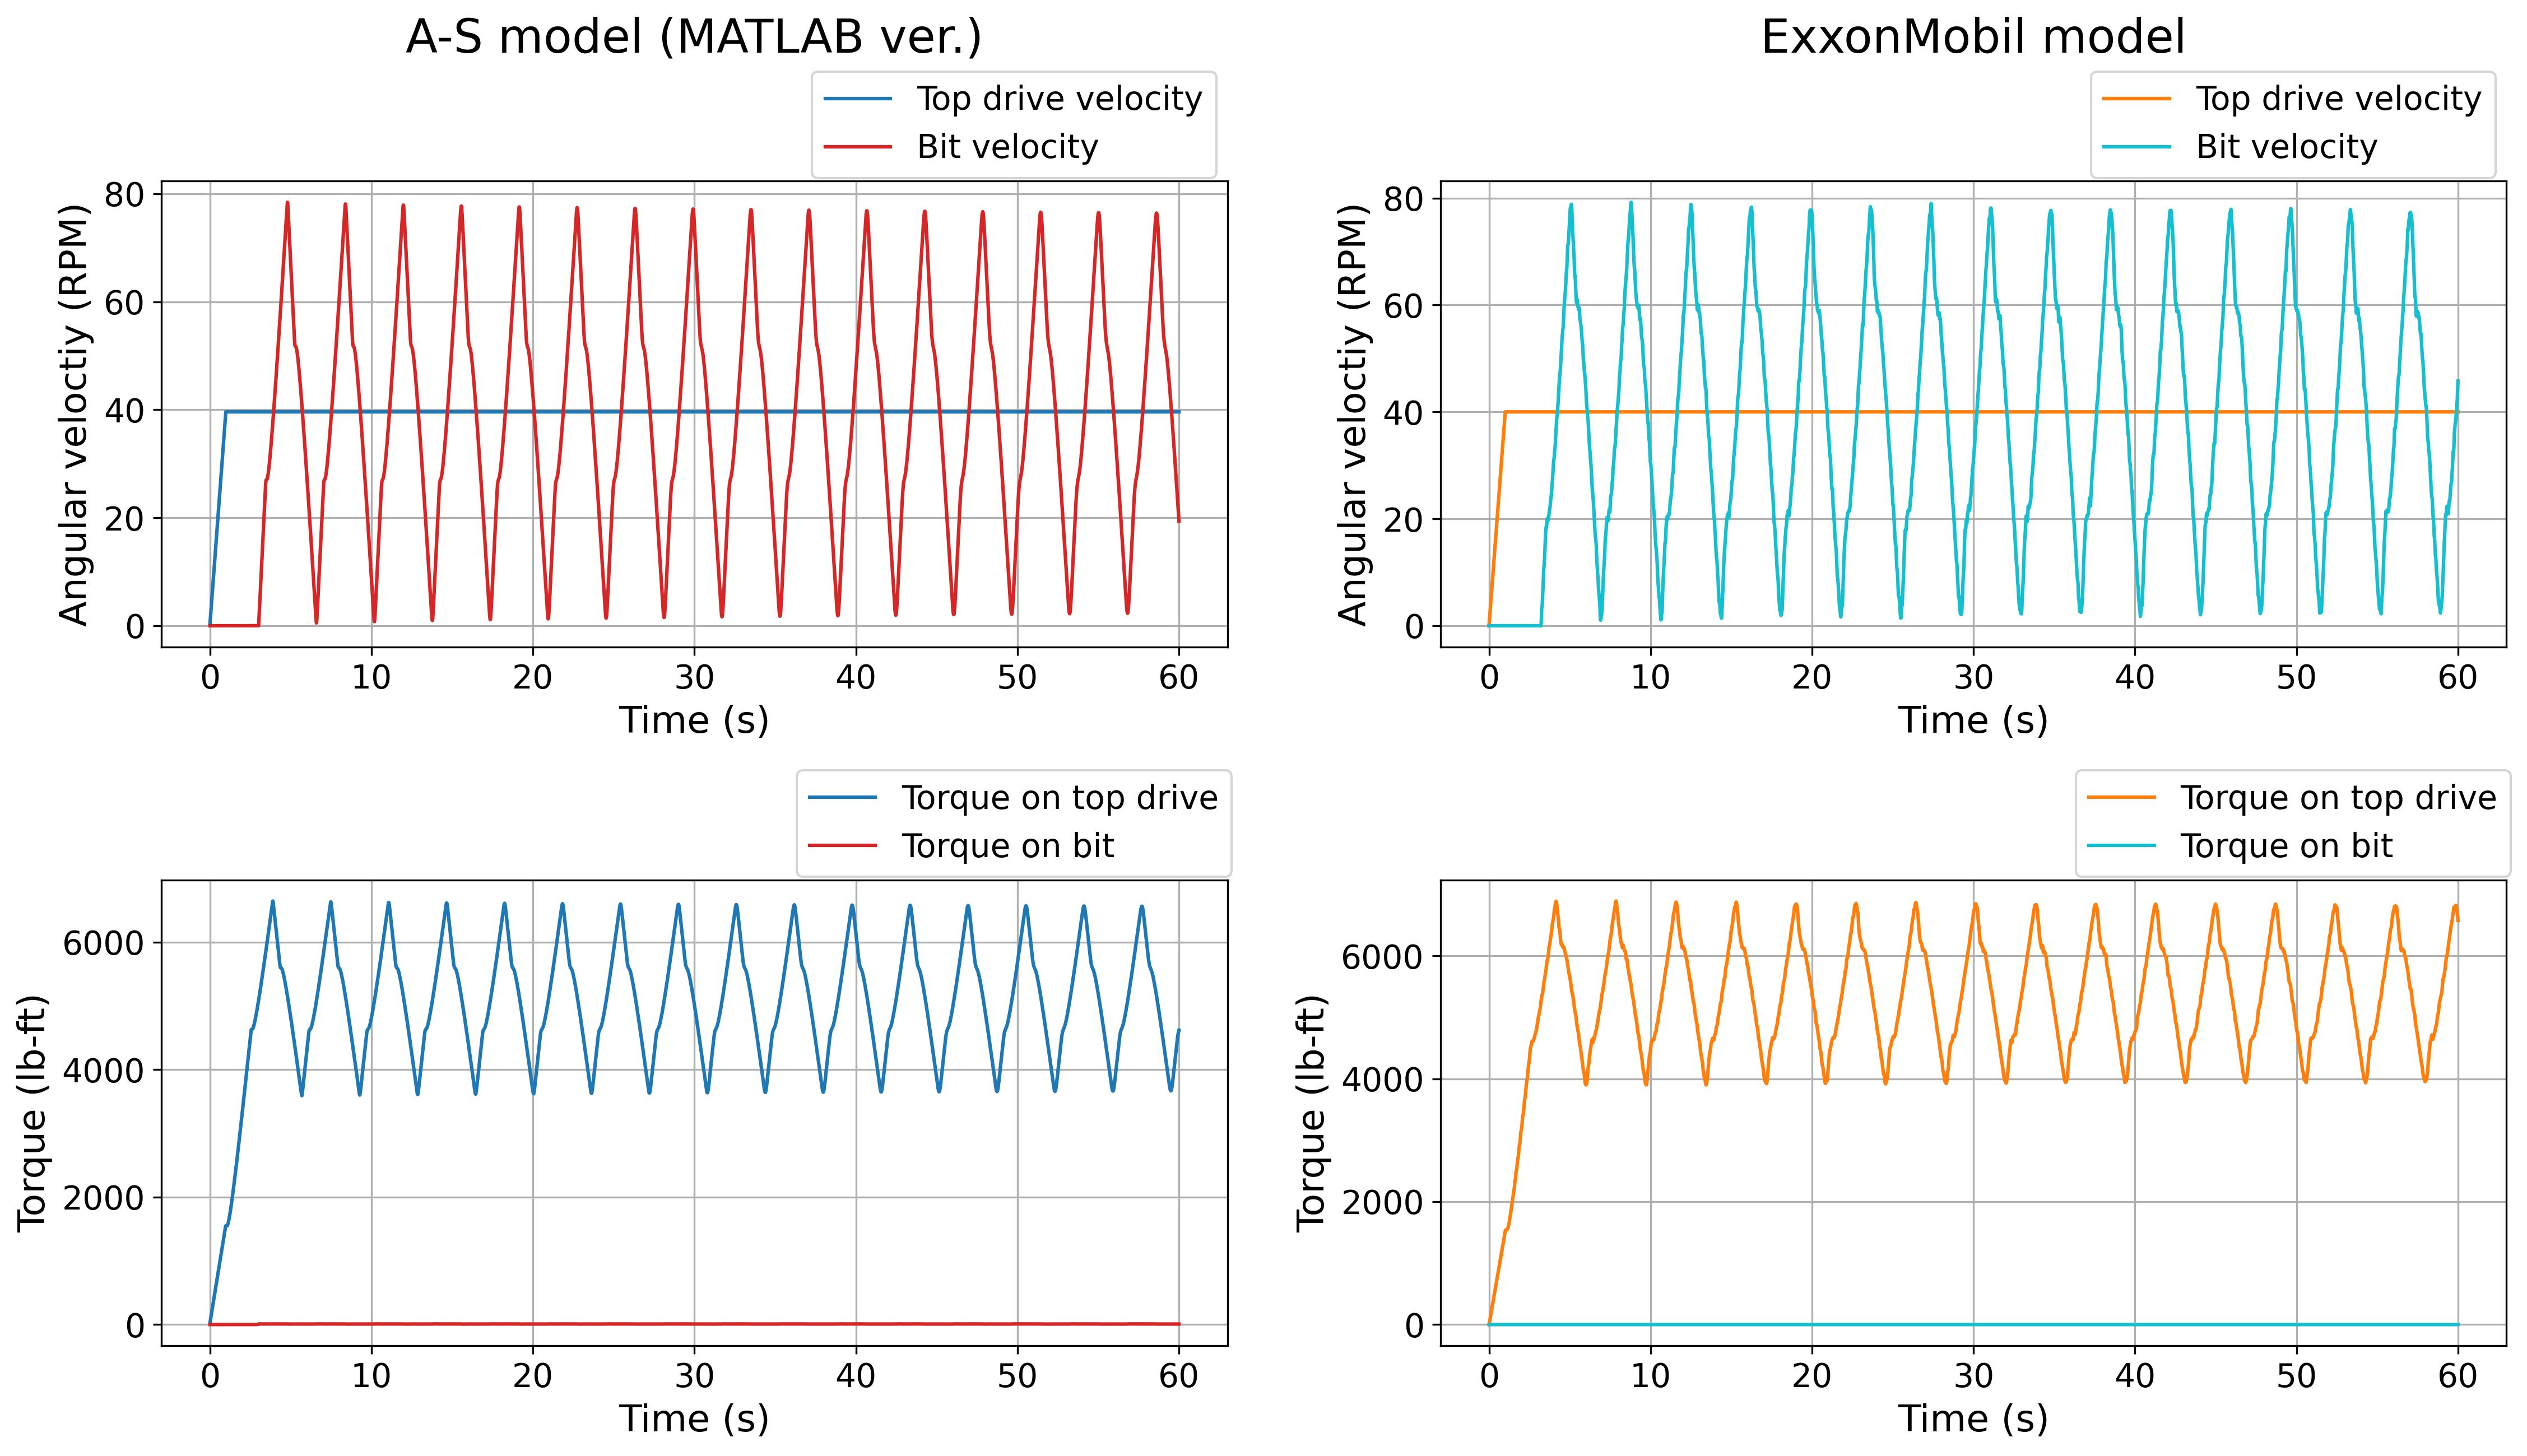
\includegraphics[width=6.5in]{output_figureTestCase2_1}
  \caption{}\label{figure_testcase2_1}
\end{figure}

\begin{figure}
  \centering
  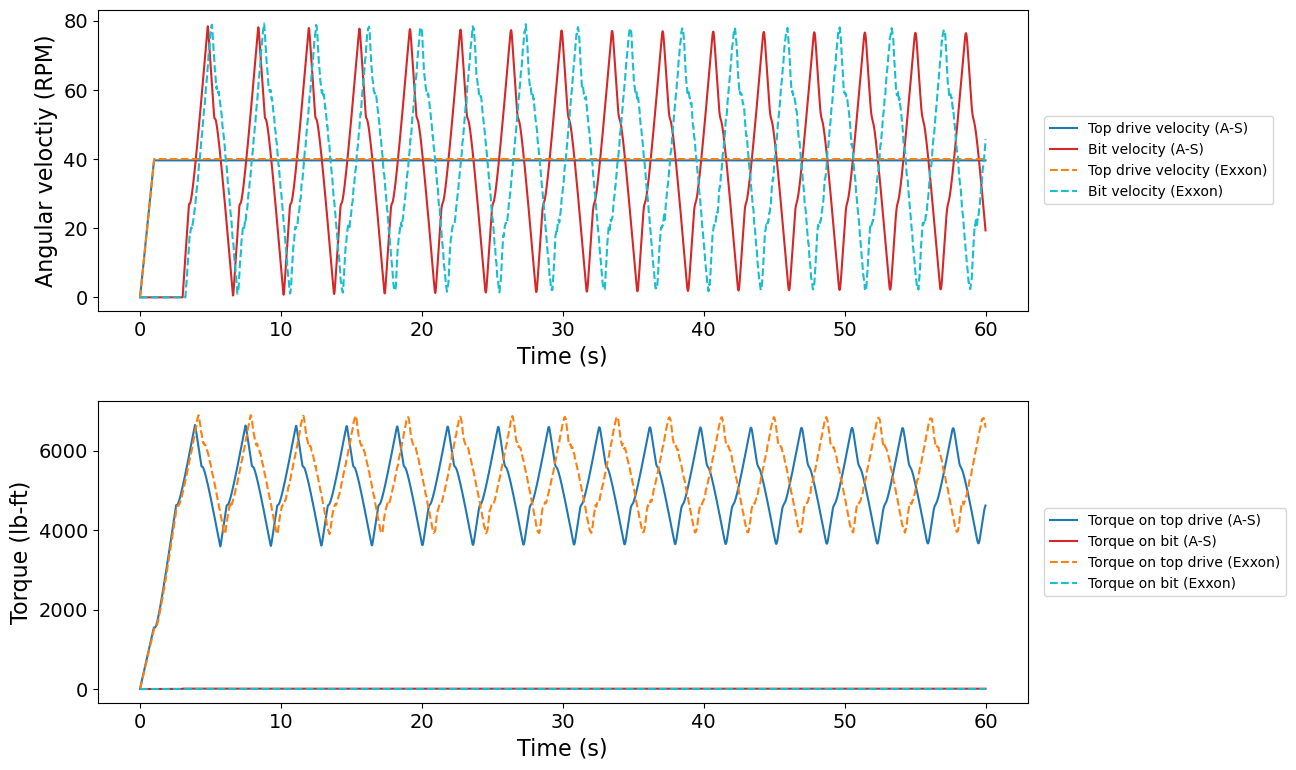
\includegraphics[width=6.5in]{overlapped_figureTestCase2_1}
  \caption{}\label{figure_testcase2_1_overlapped}
\end{figure}

\begin{figure}
  \centering
  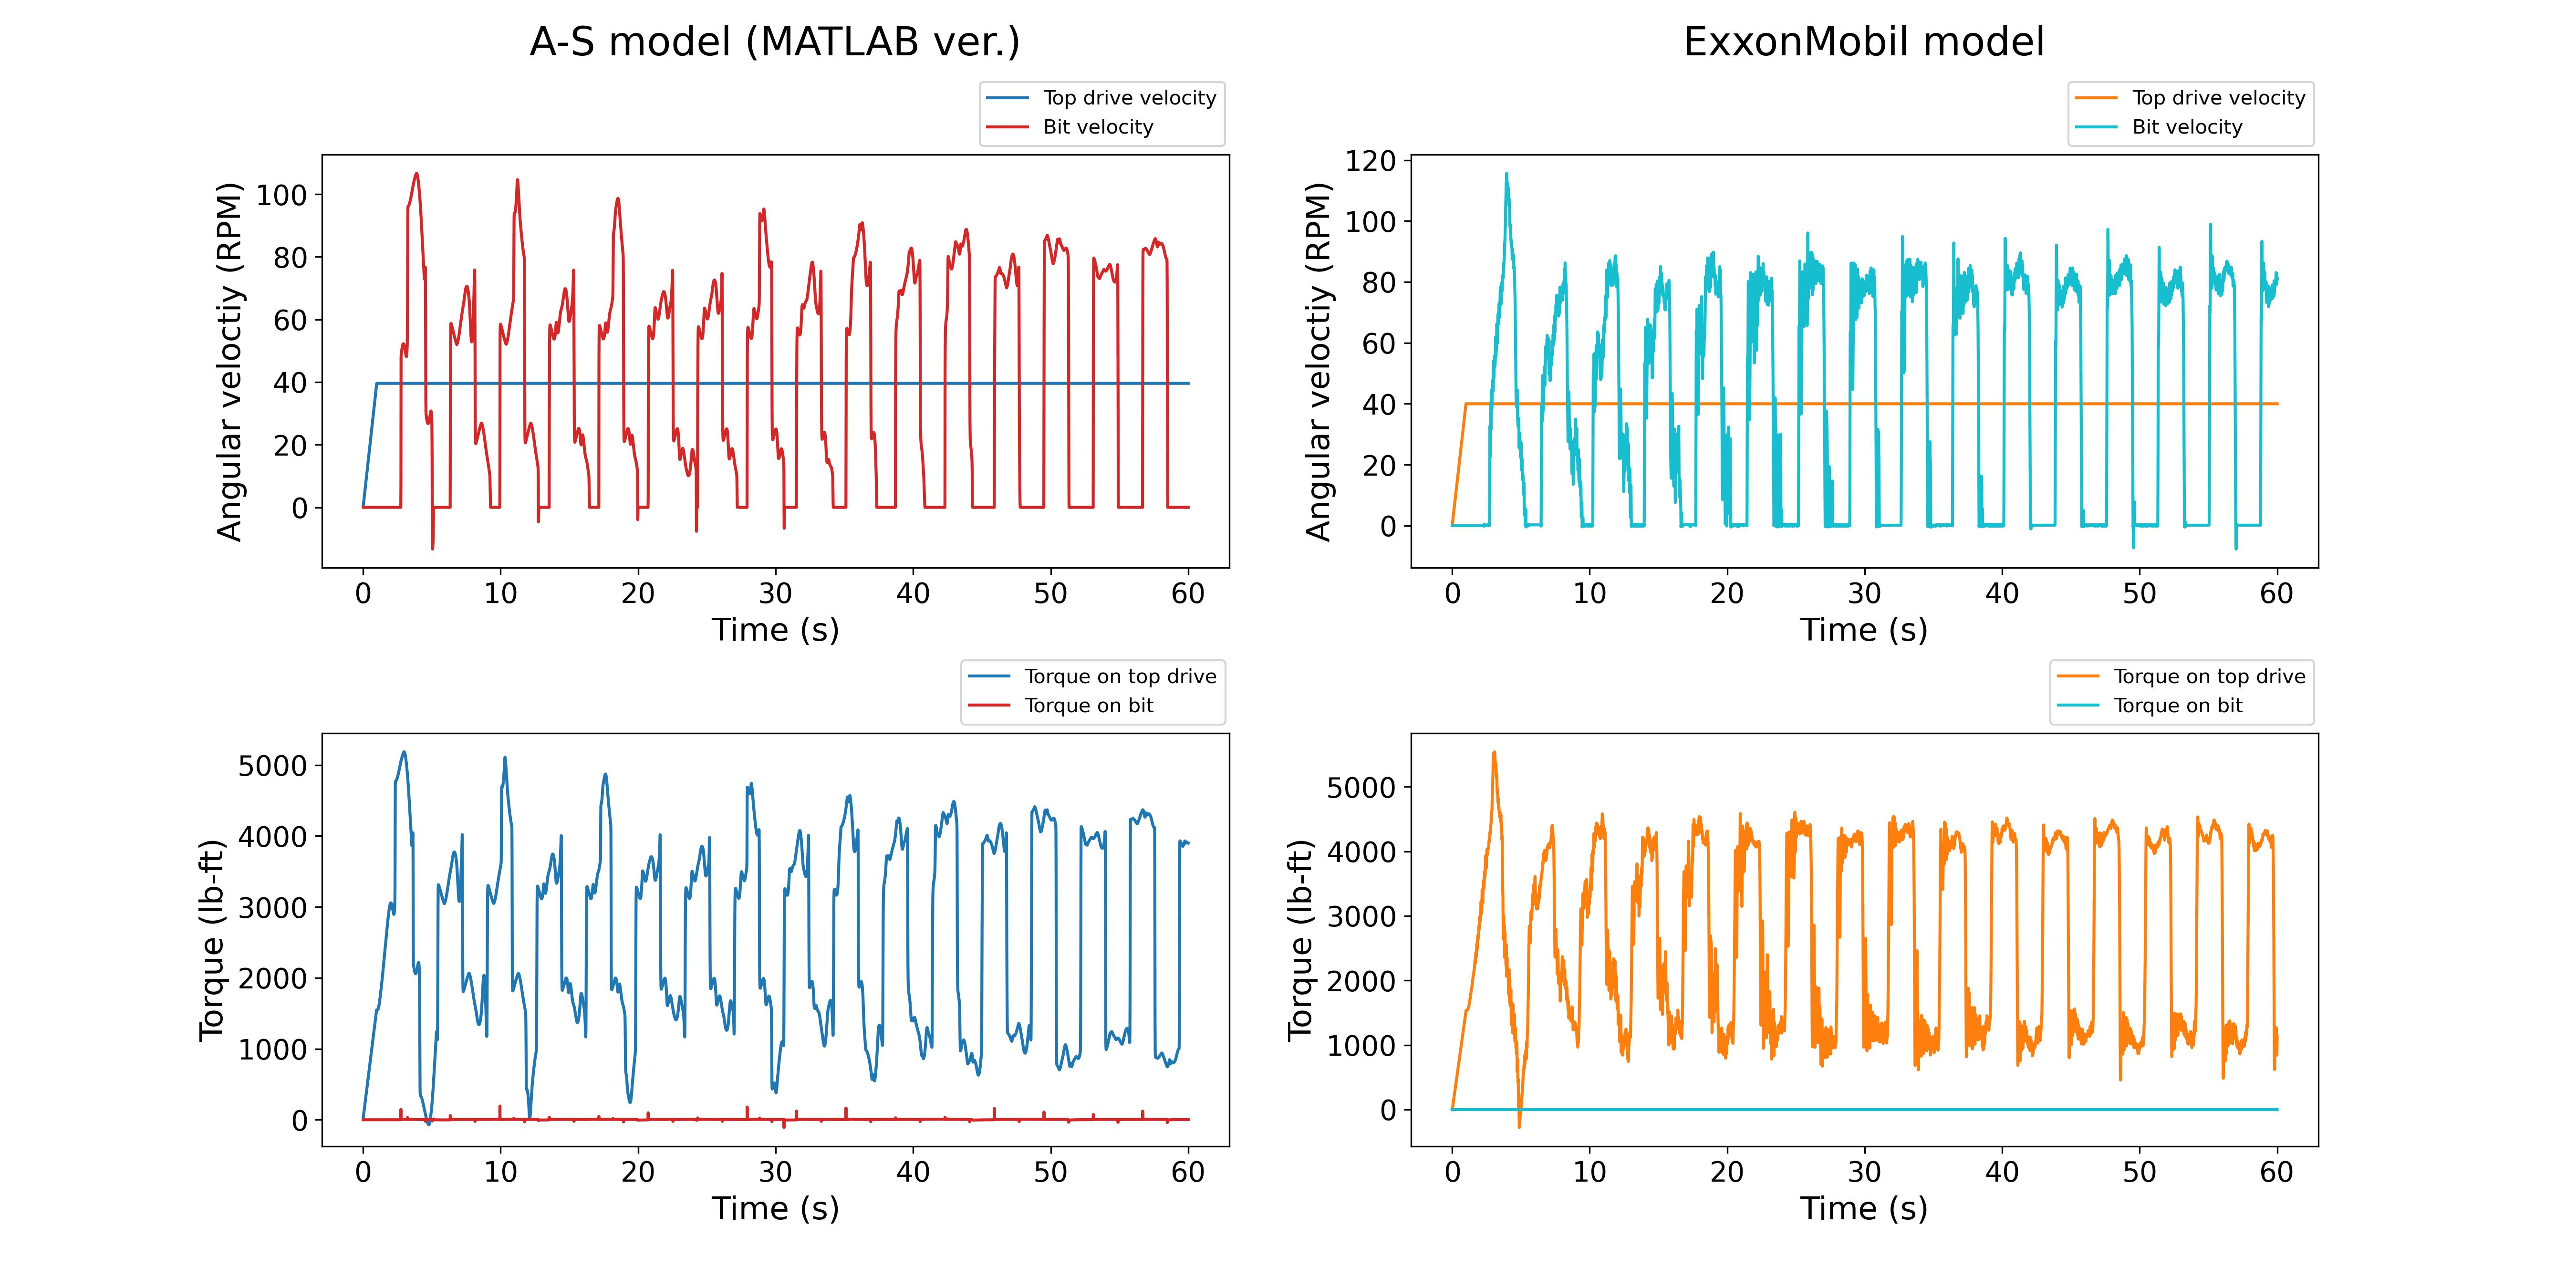
\includegraphics[width=6.5in]{output_figureTestCase2_2}
  \caption{}\label{figure_testcase2_2}
\end{figure}

\begin{figure}
  \centering
  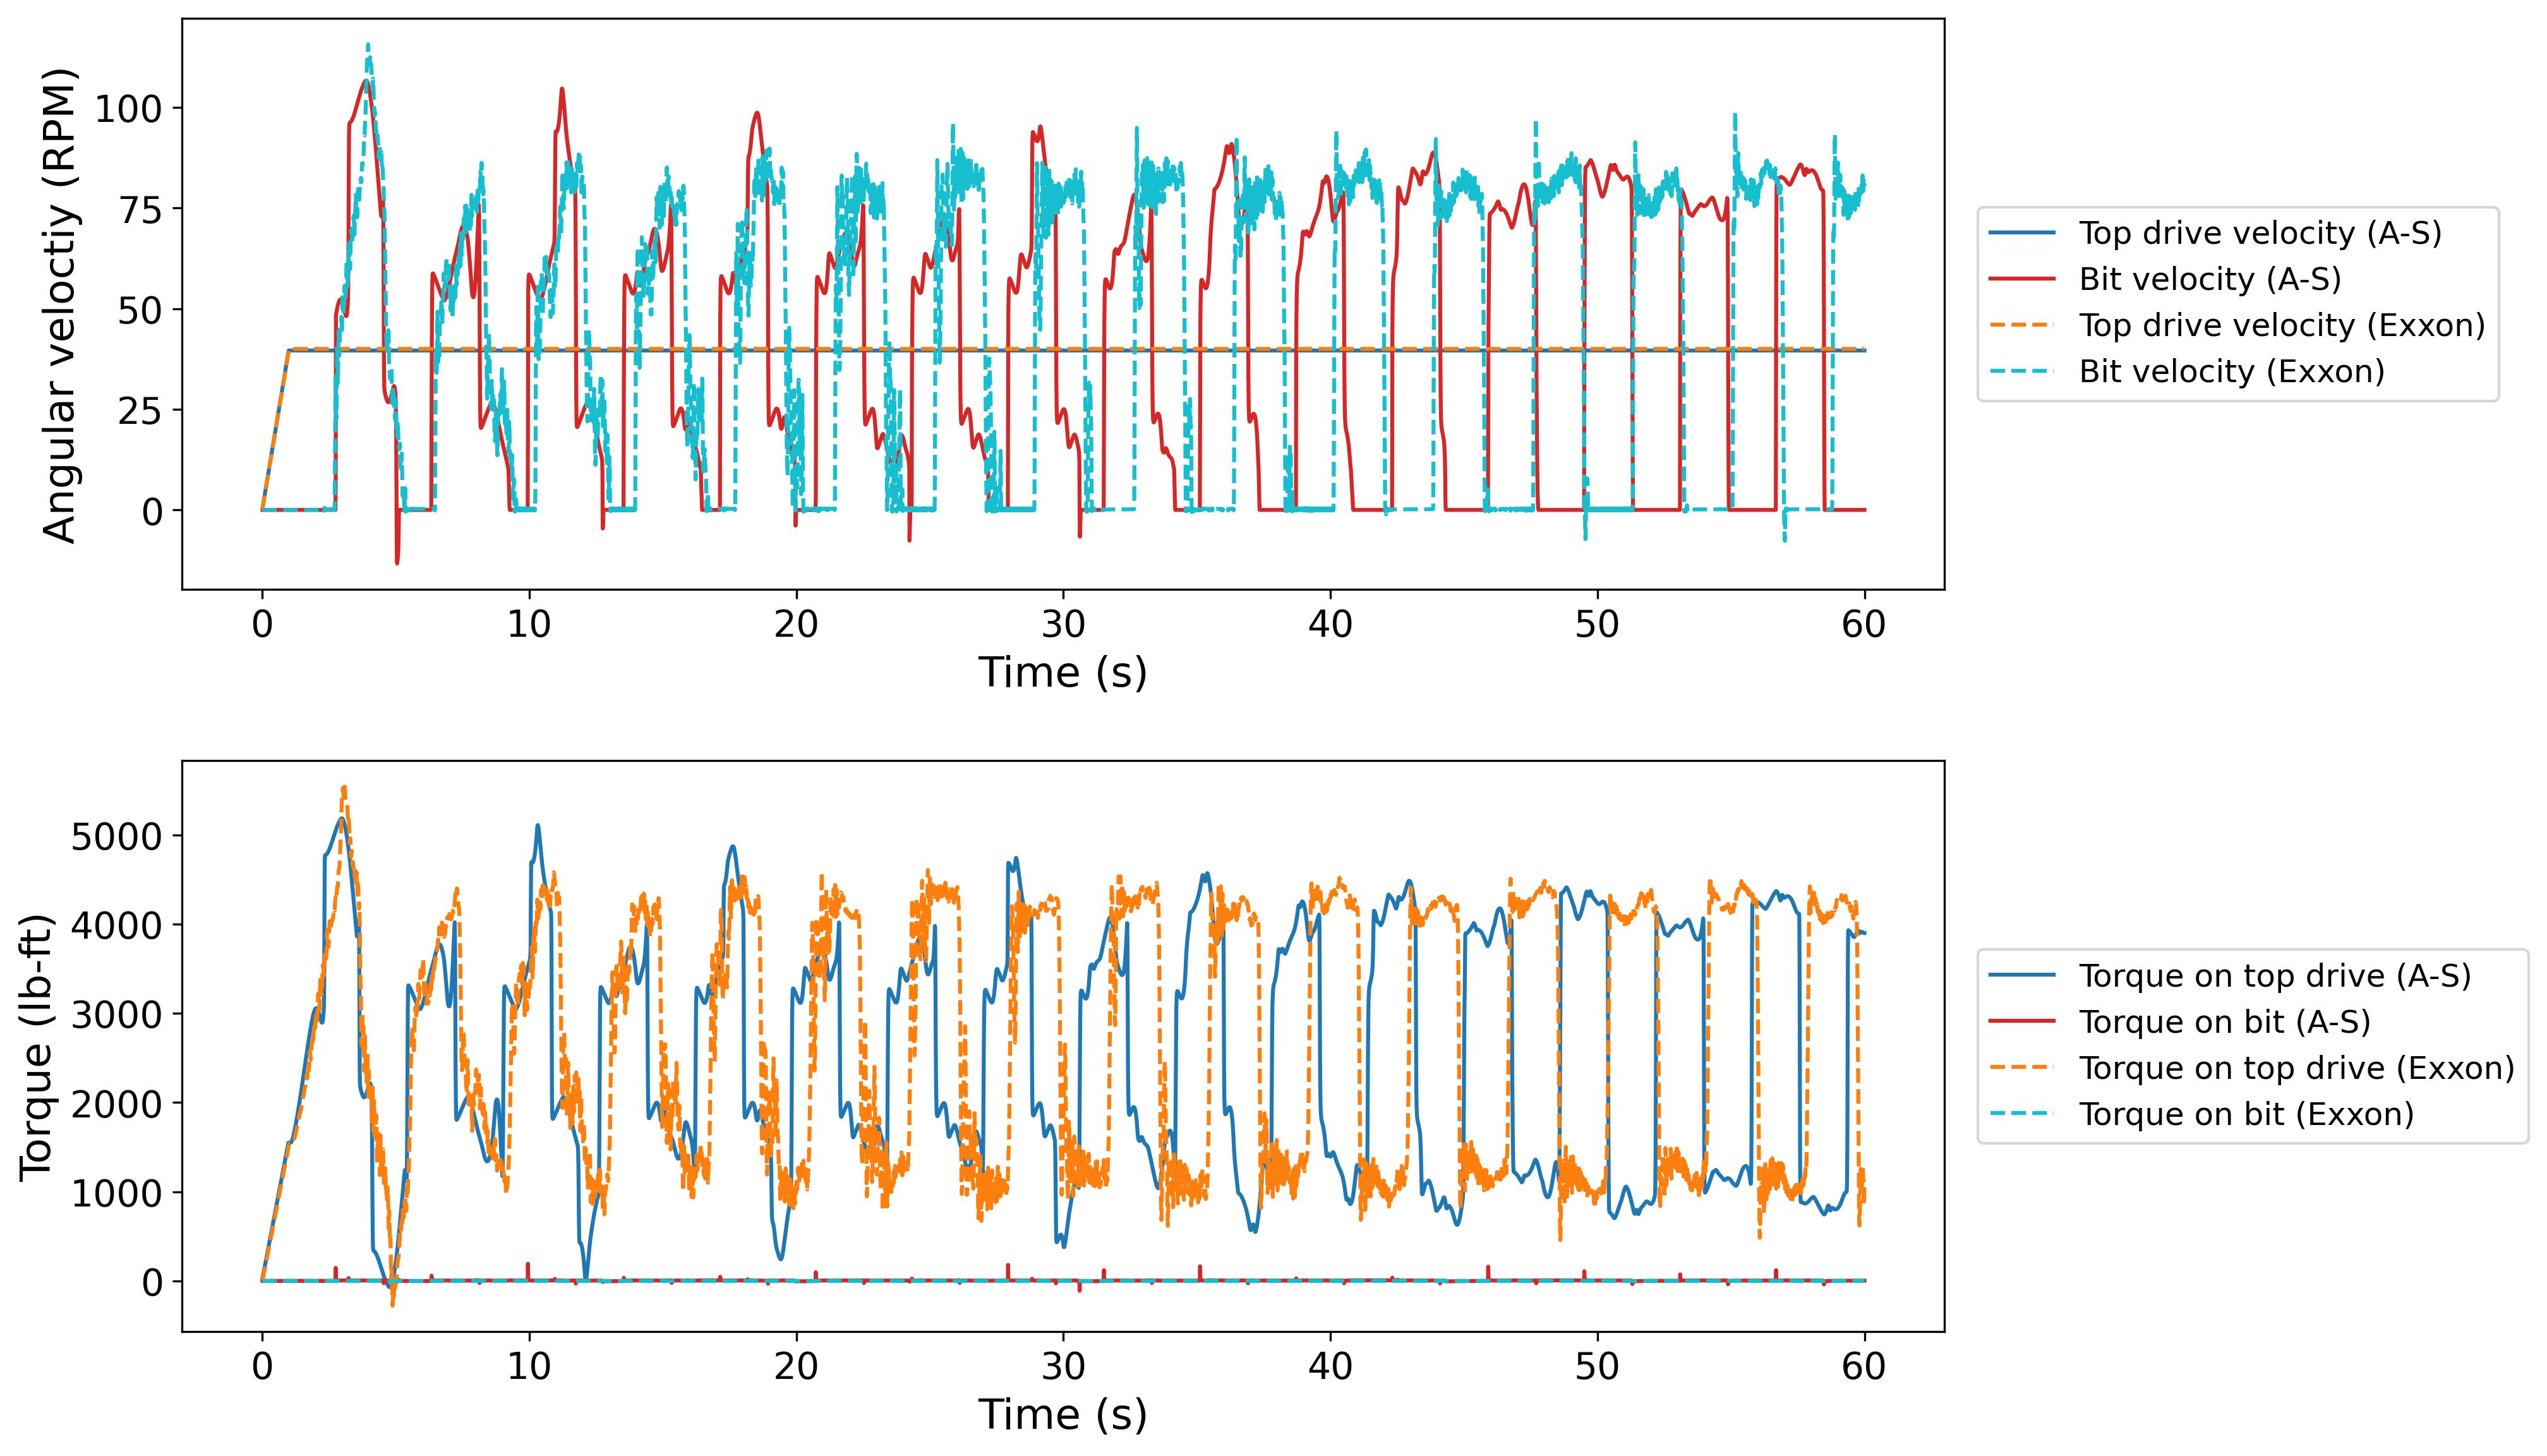
\includegraphics[width=6.5in]{overlapped_figureTestCase2_2}
  \caption{}\label{figure_testcase2_2_overlapped}
\end{figure}

\section{Test Case 3}

\begin{figure}
  \centering
  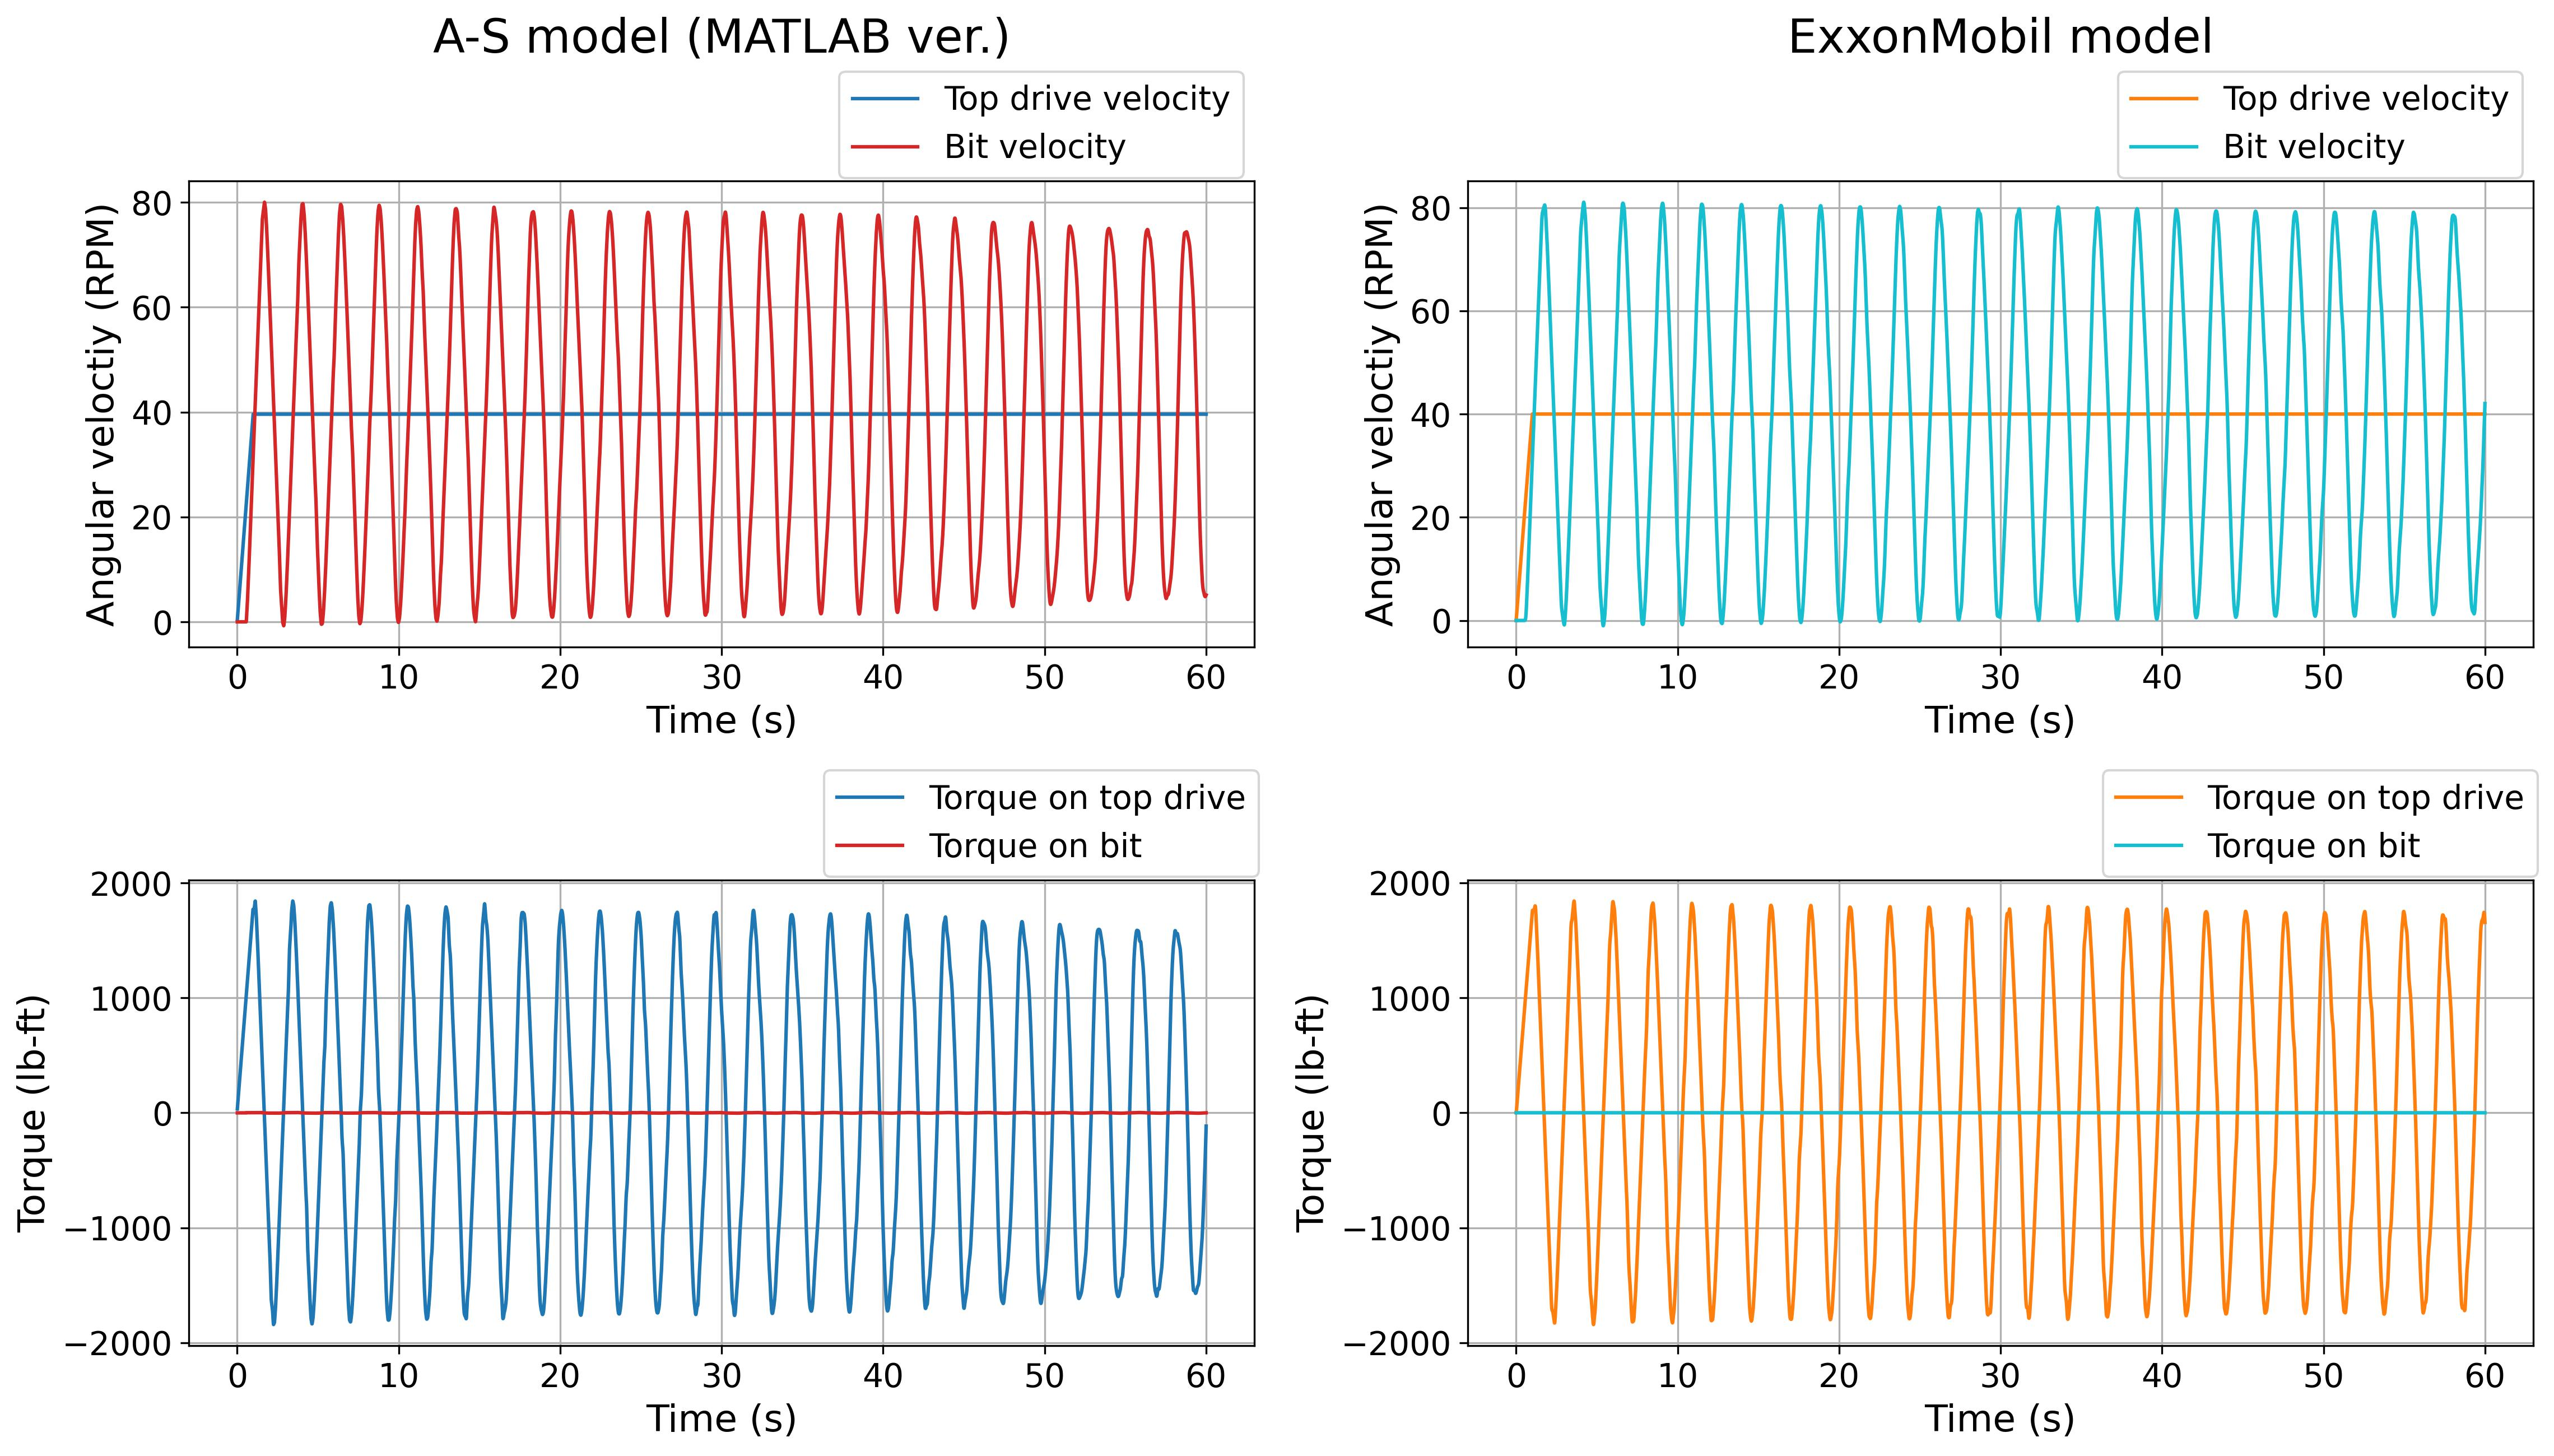
\includegraphics[width=6.5in]{output_figureTestCase3}
  \caption{}\label{figure_testcase3}
\end{figure}
\begin{figure}
  \centering
  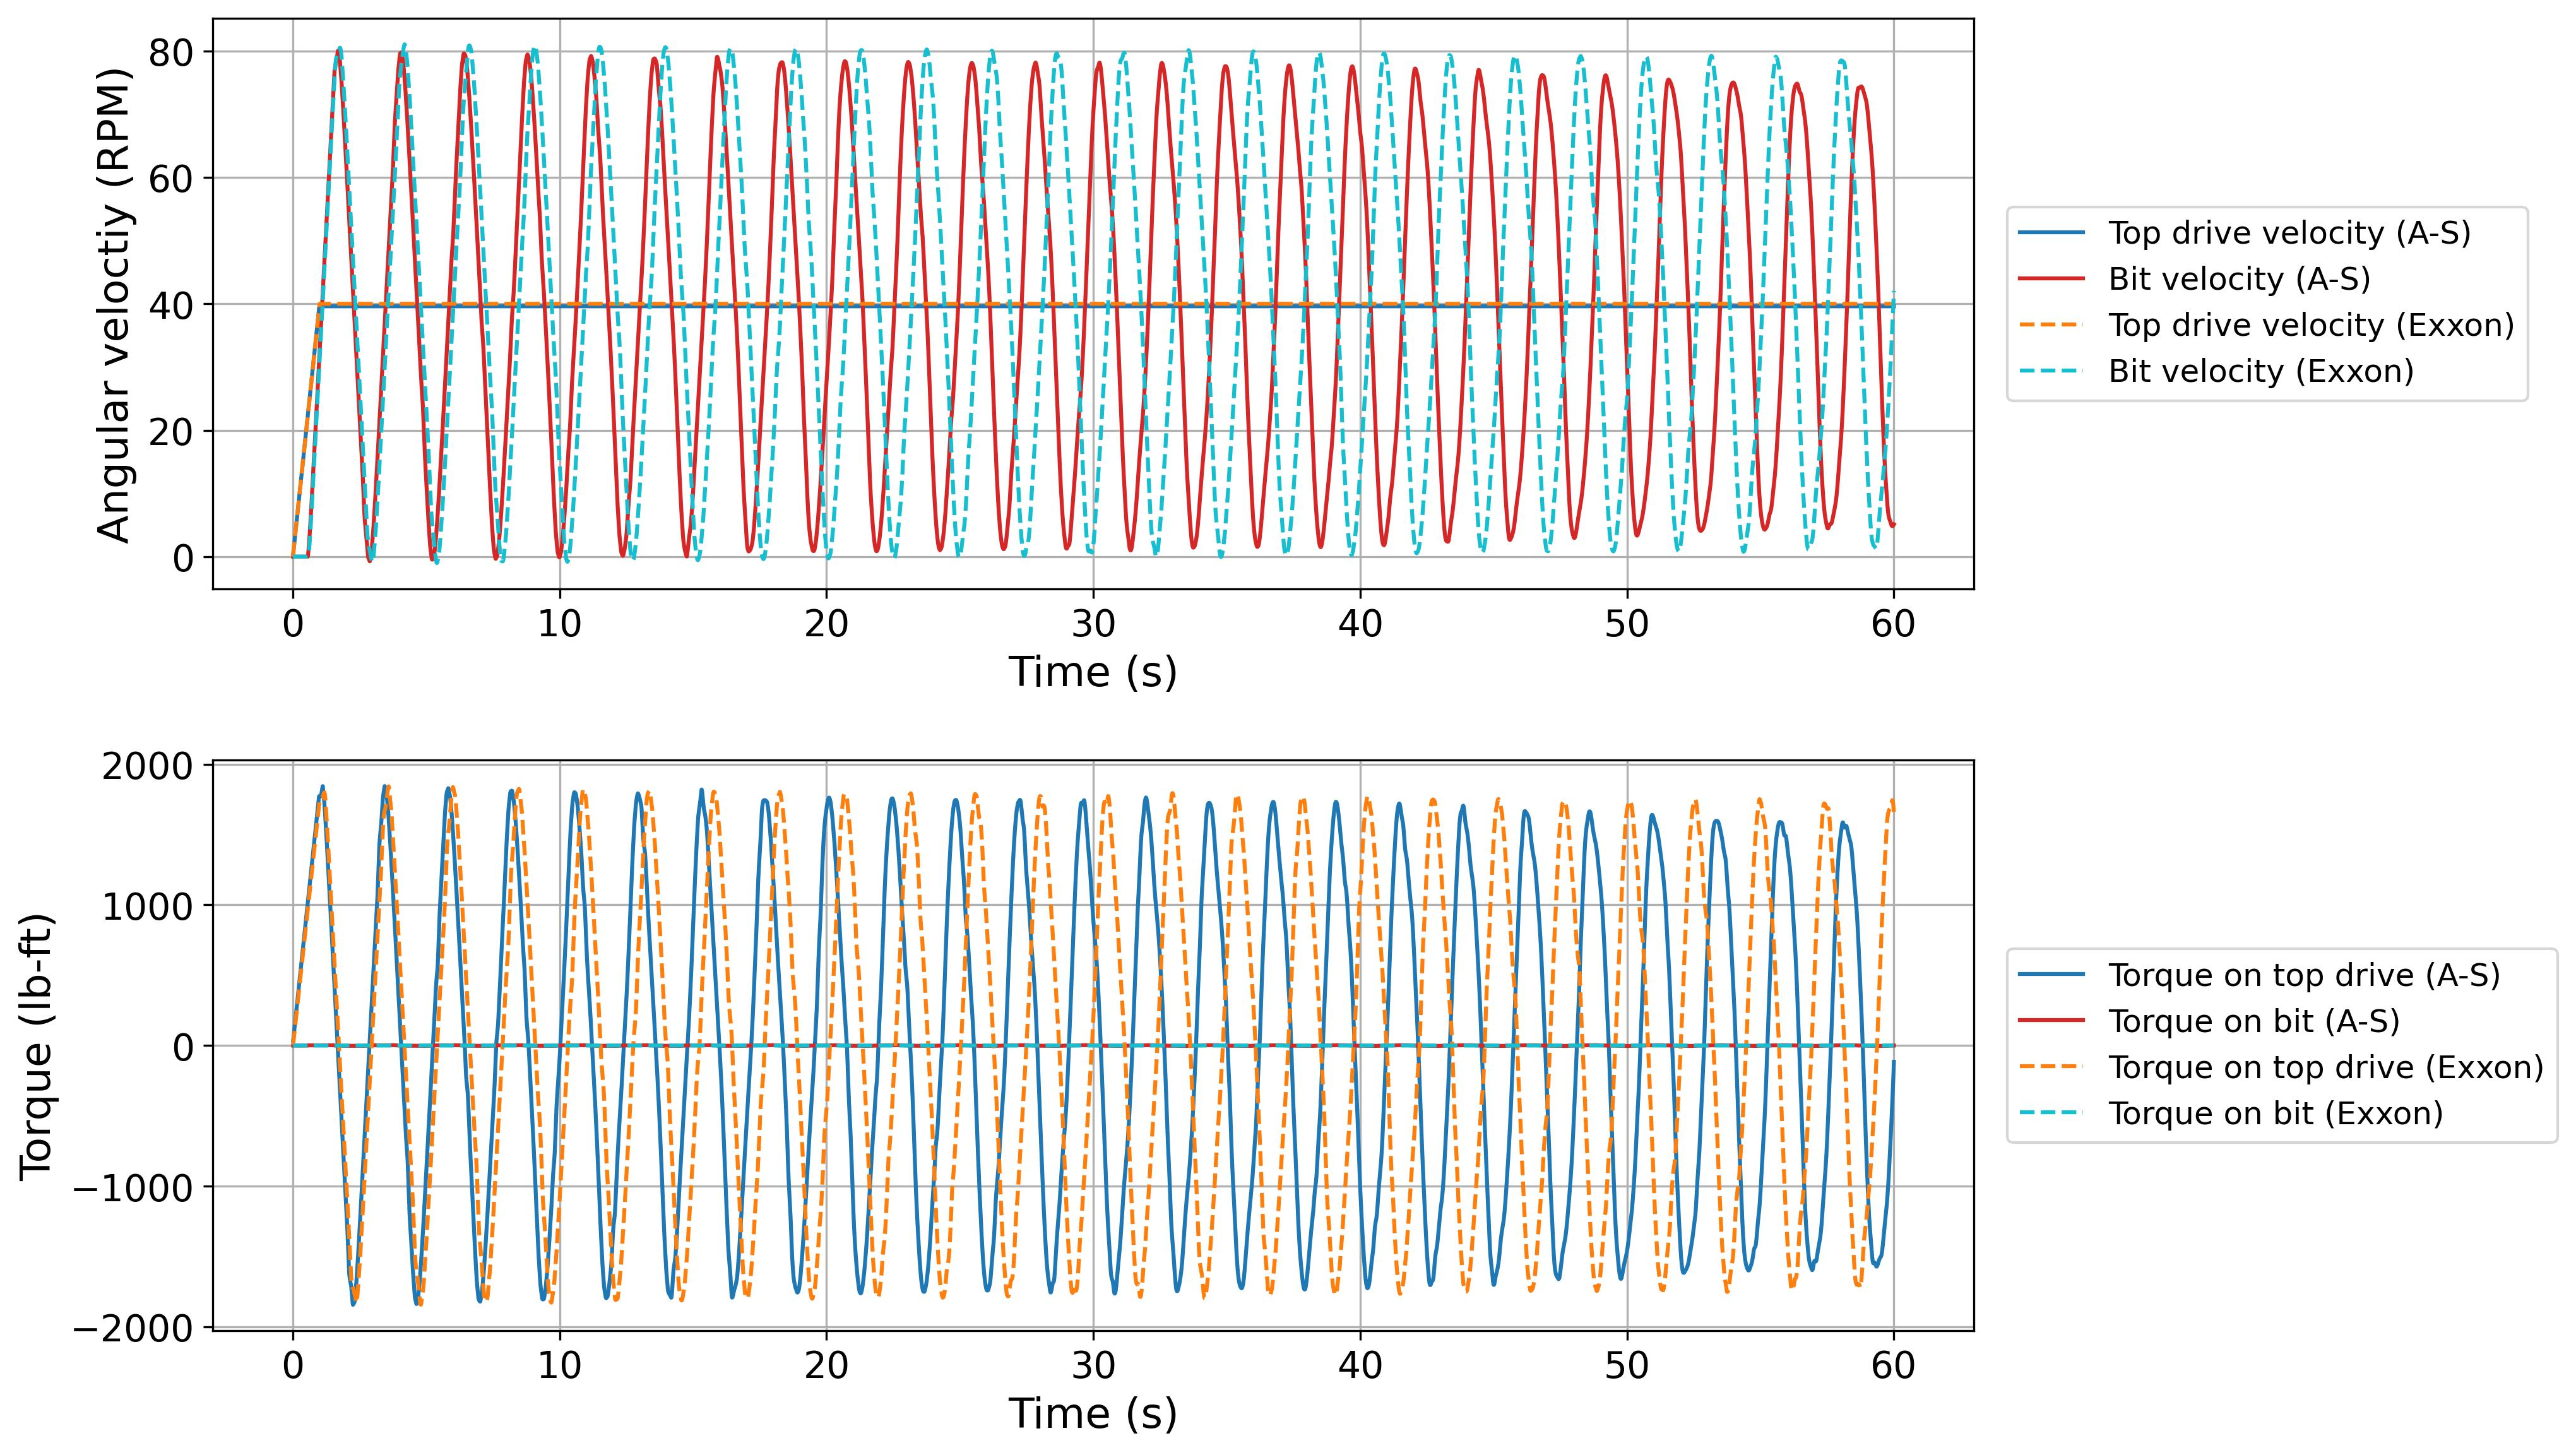
\includegraphics[width=6.5in]{overlapped_figureTestCase3}
  \caption{}\label{figure_testcase3_overlapped}
\end{figure}

\section{Test Case 4}

\begin{figure}
  \centering
  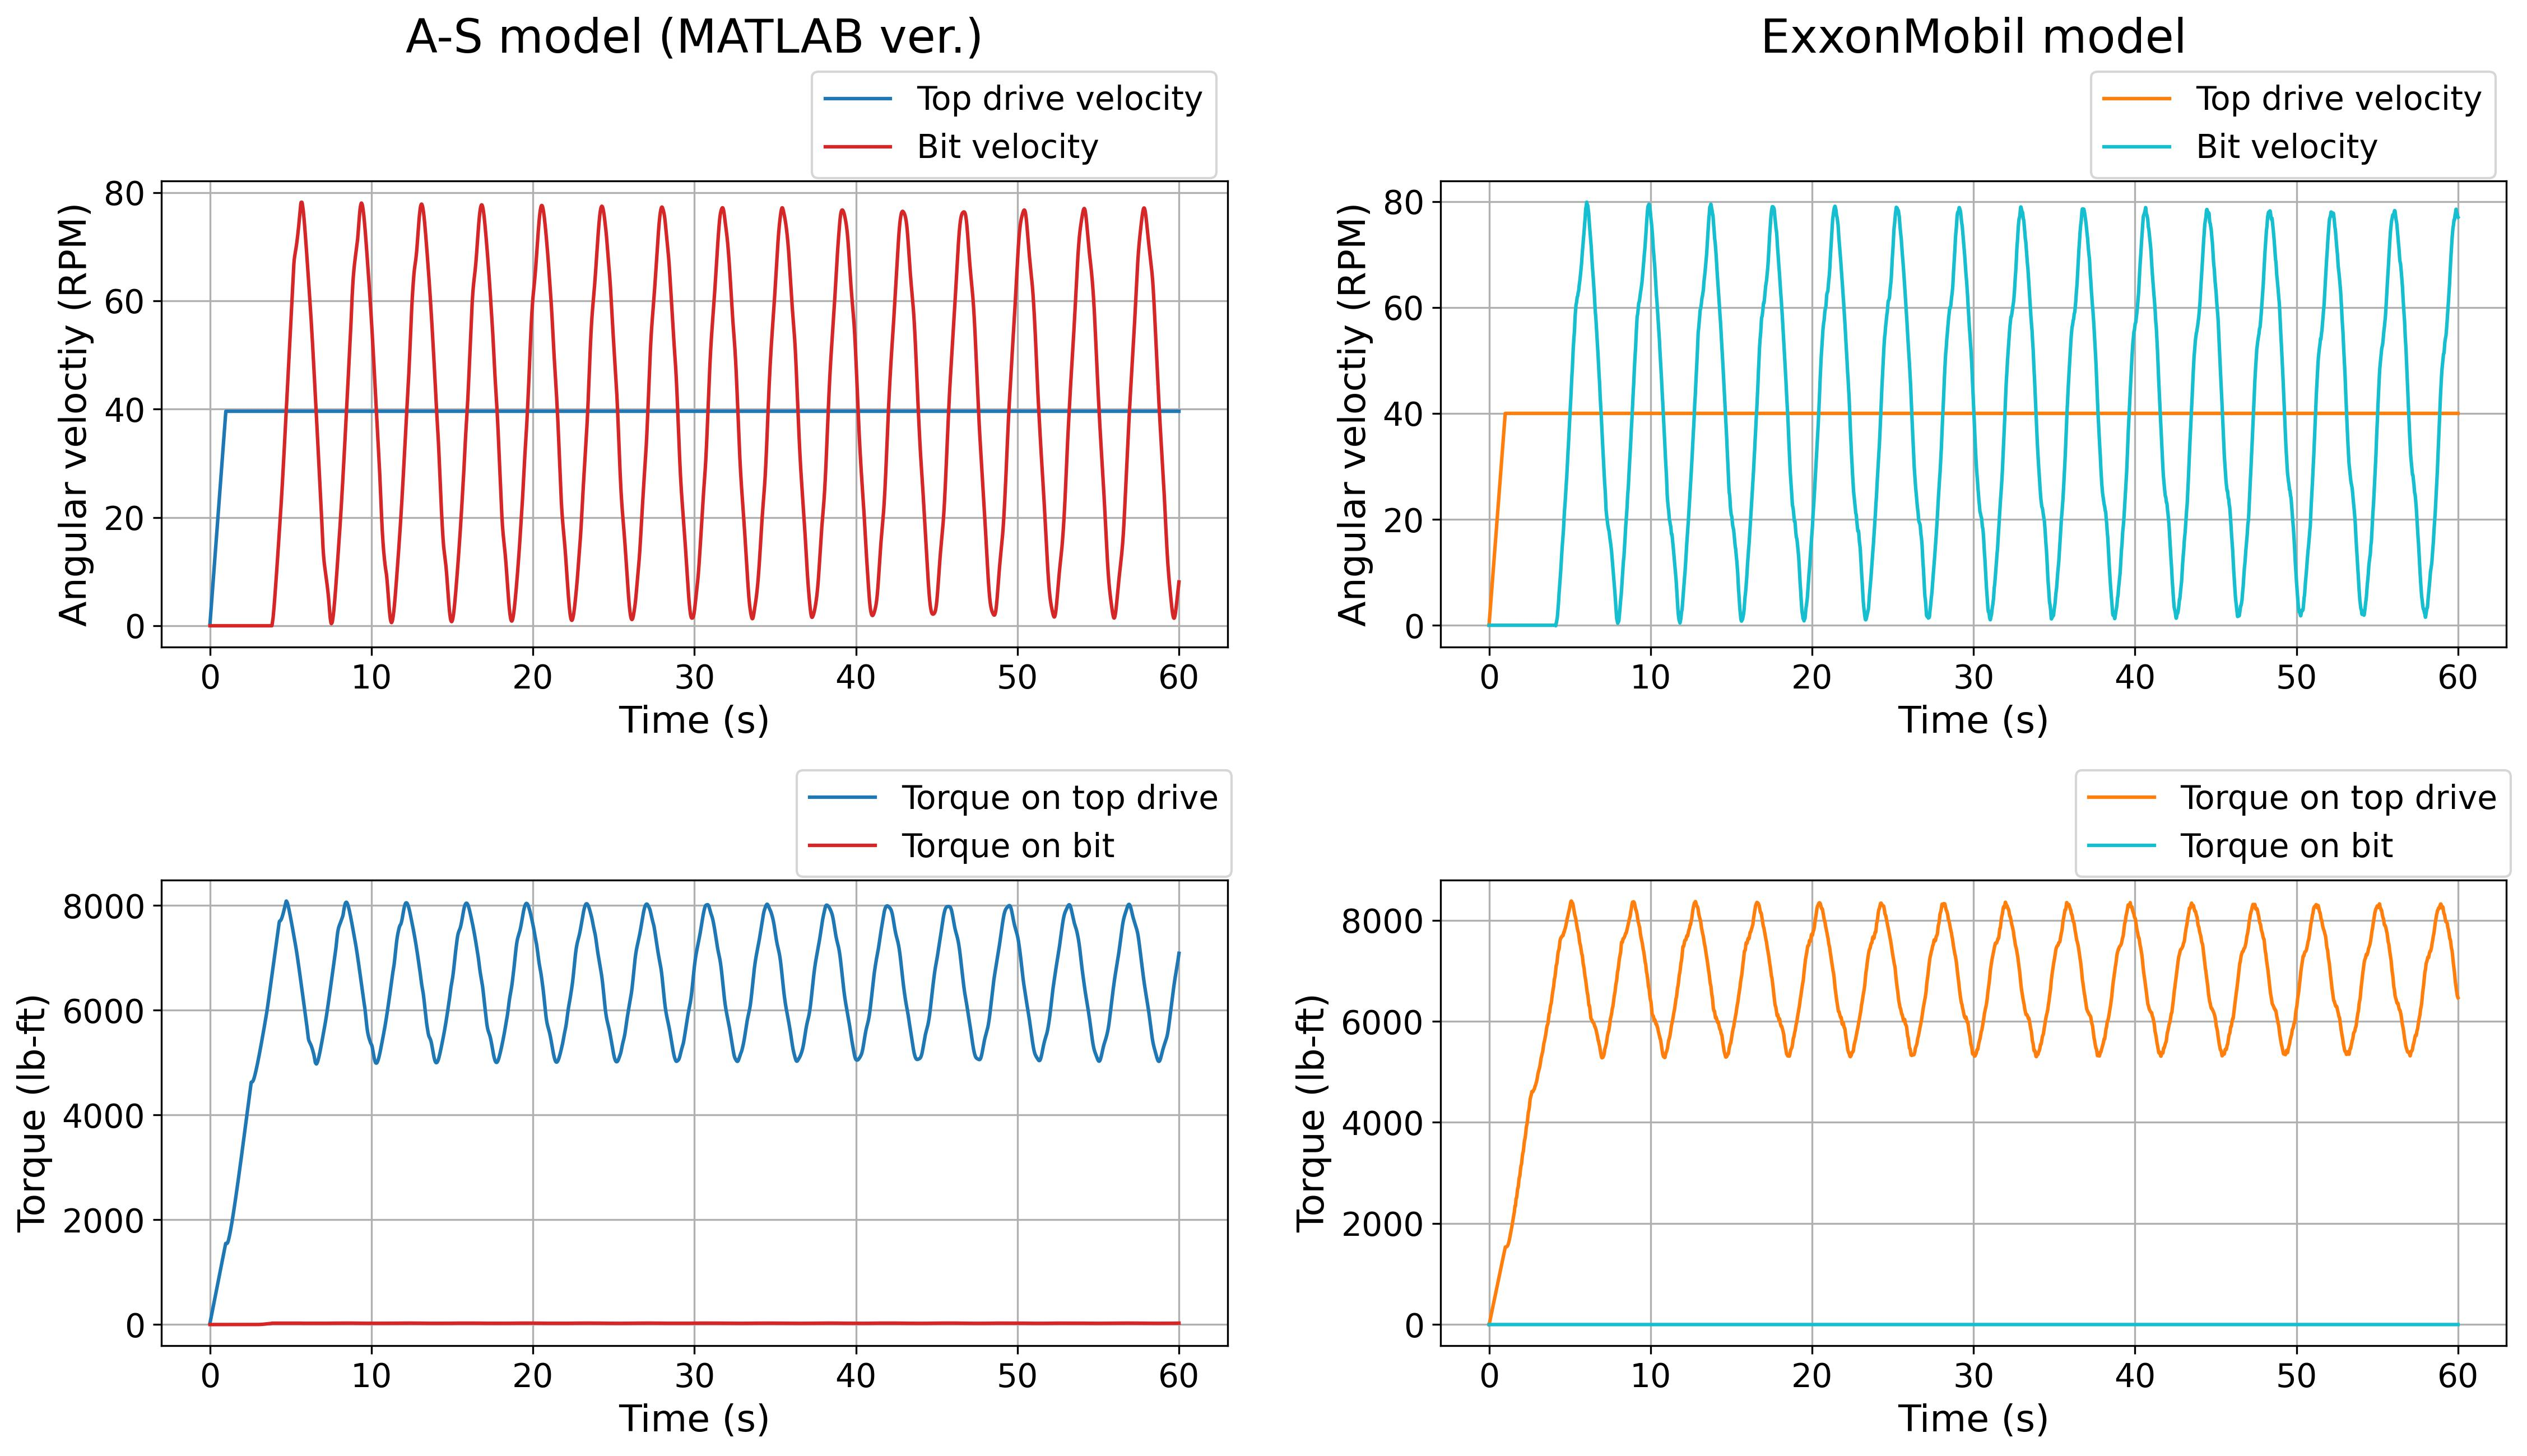
\includegraphics[width=6.5in]{output_figureTestCase4_1}
  \caption{}\label{figure_testcase4_1}
\end{figure}

\begin{figure}
  \centering
  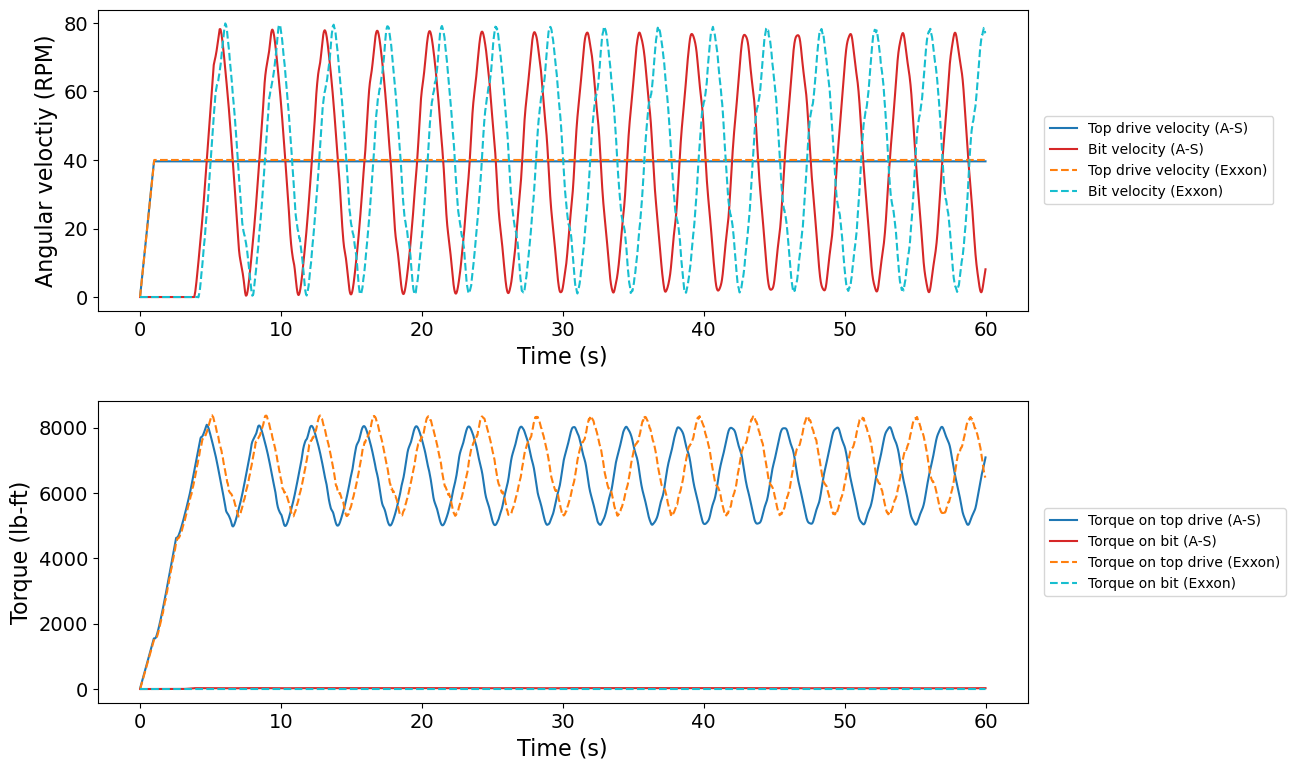
\includegraphics[width=6.5in]{overlapped_figureTestCase4_1}
  \caption{}\label{figure_testcase4_1_overlapped}
\end{figure}

\begin{figure}
  \centering
  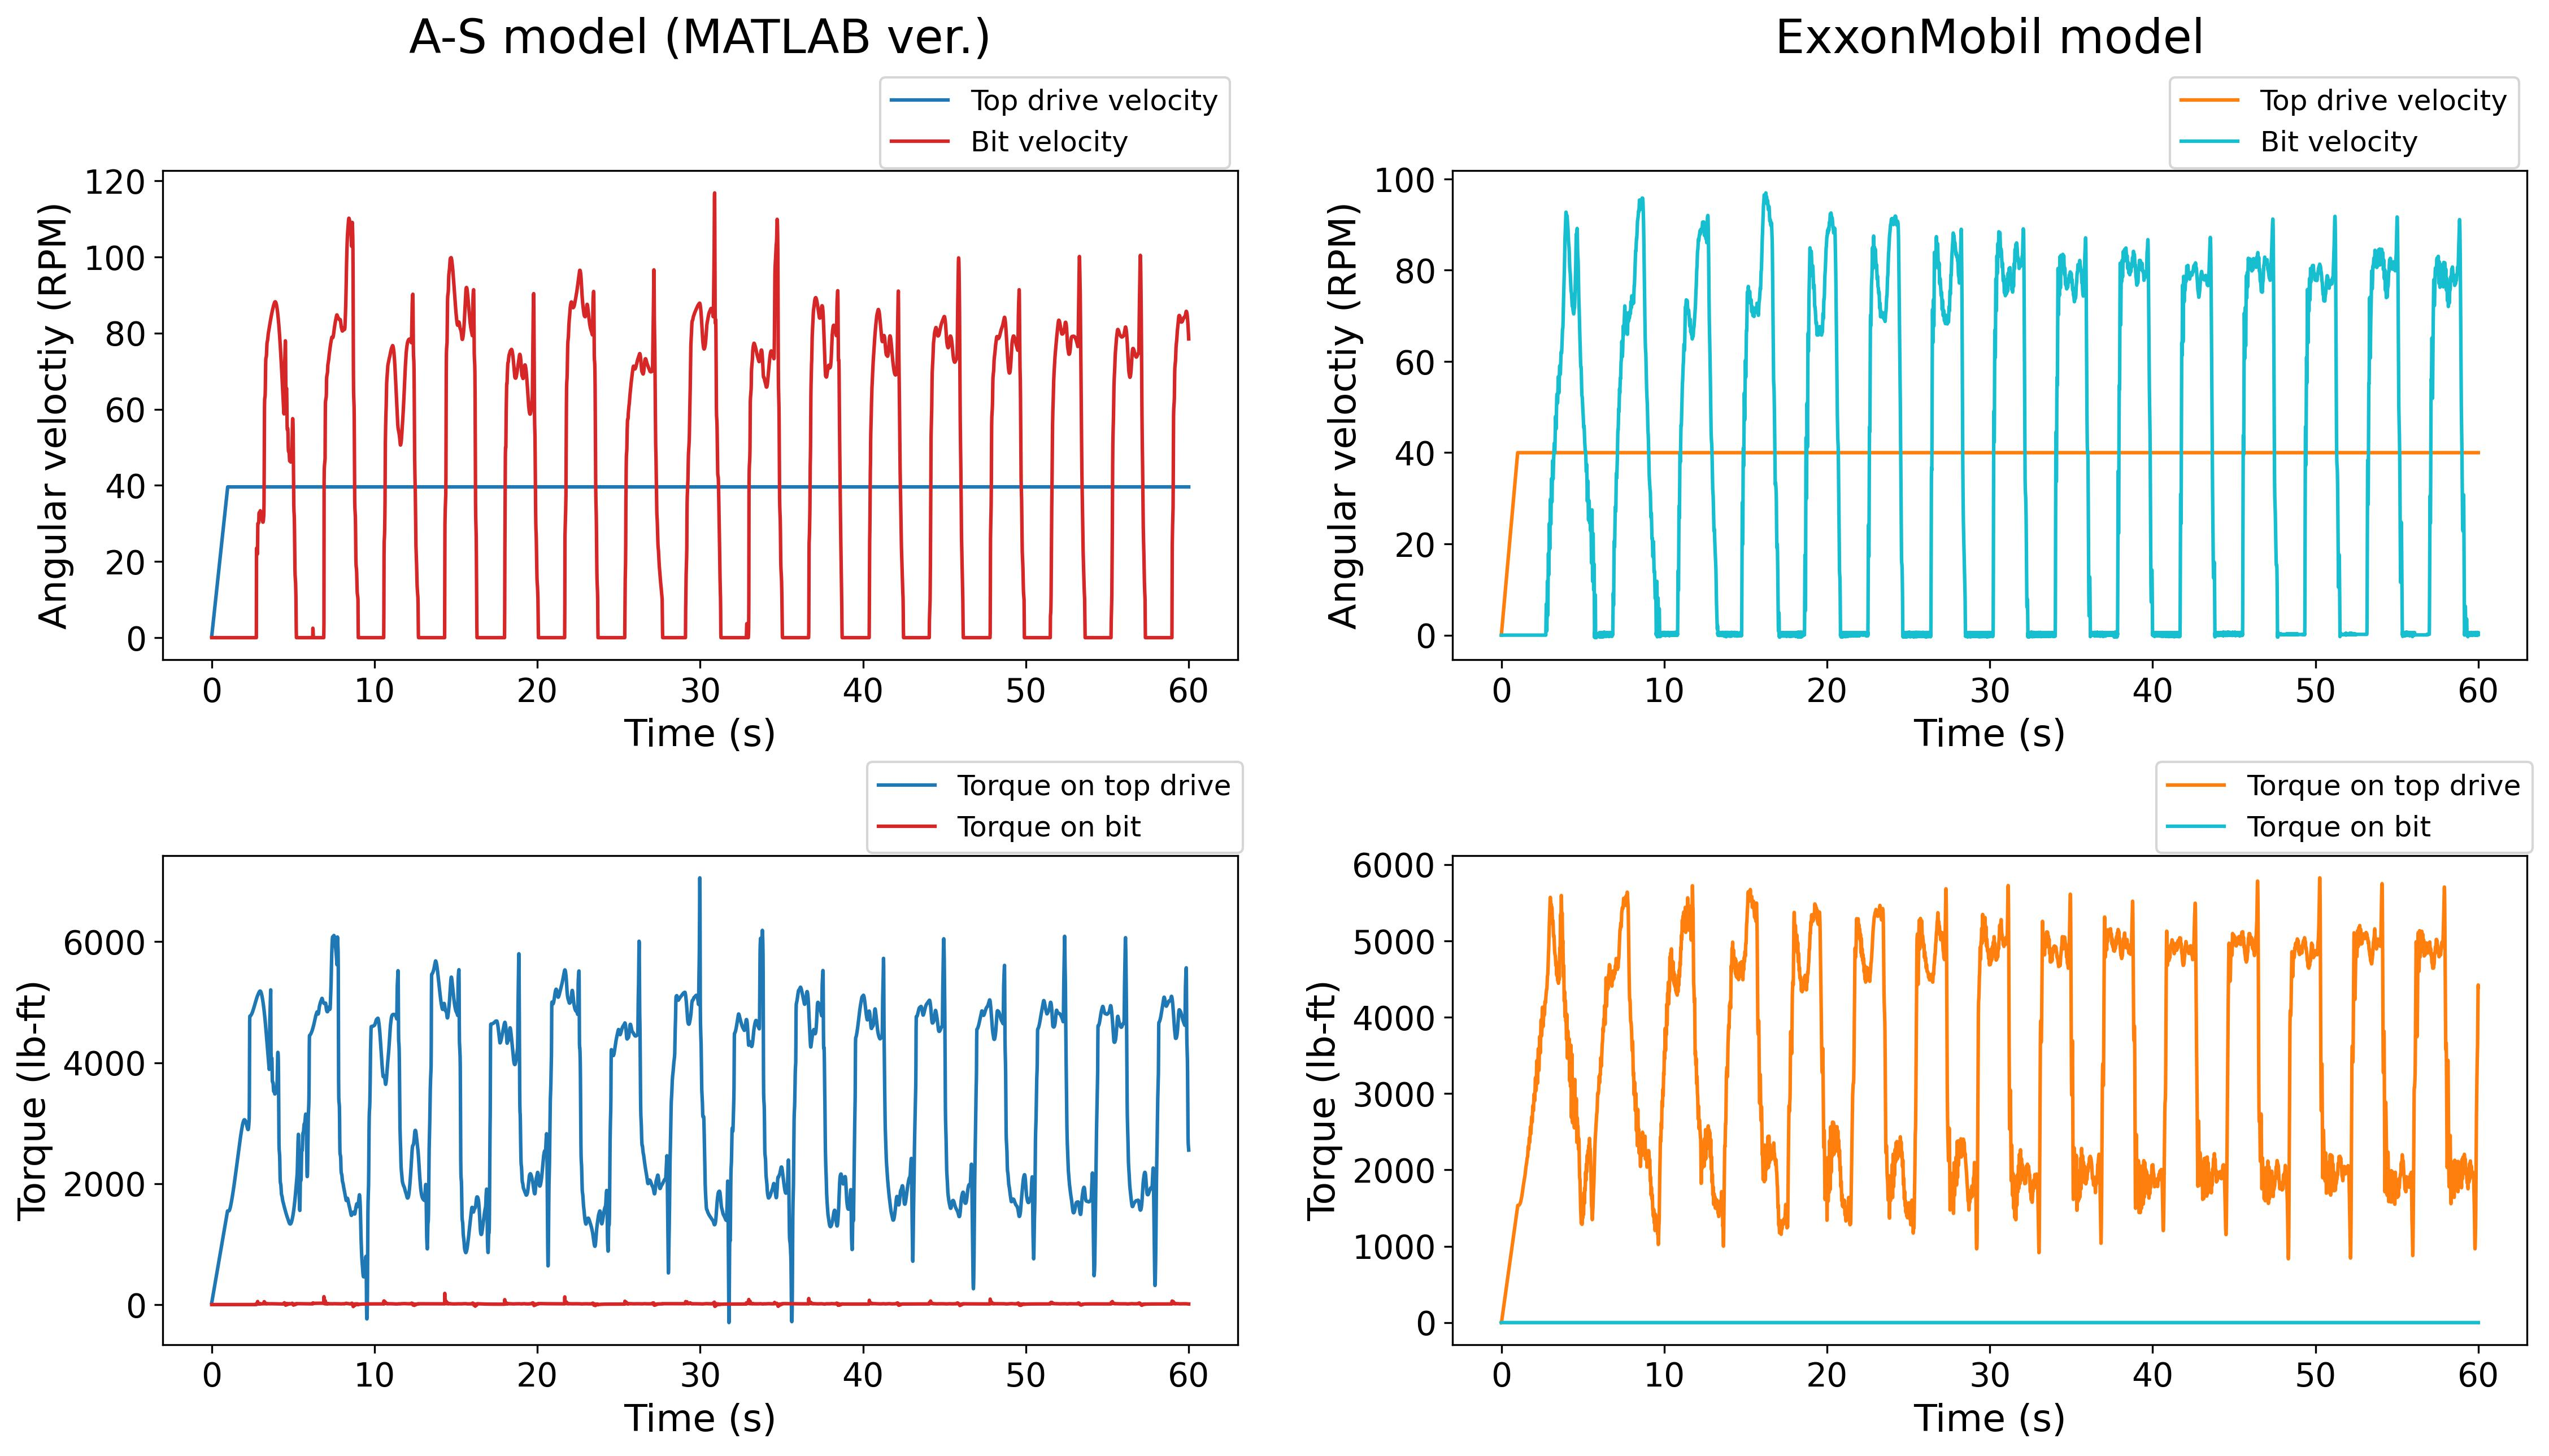
\includegraphics[width=6.5in]{output_figureTestCase4_2}
  \caption{}\label{figure_testcase4_2}
\end{figure}

\begin{figure}
  \centering
  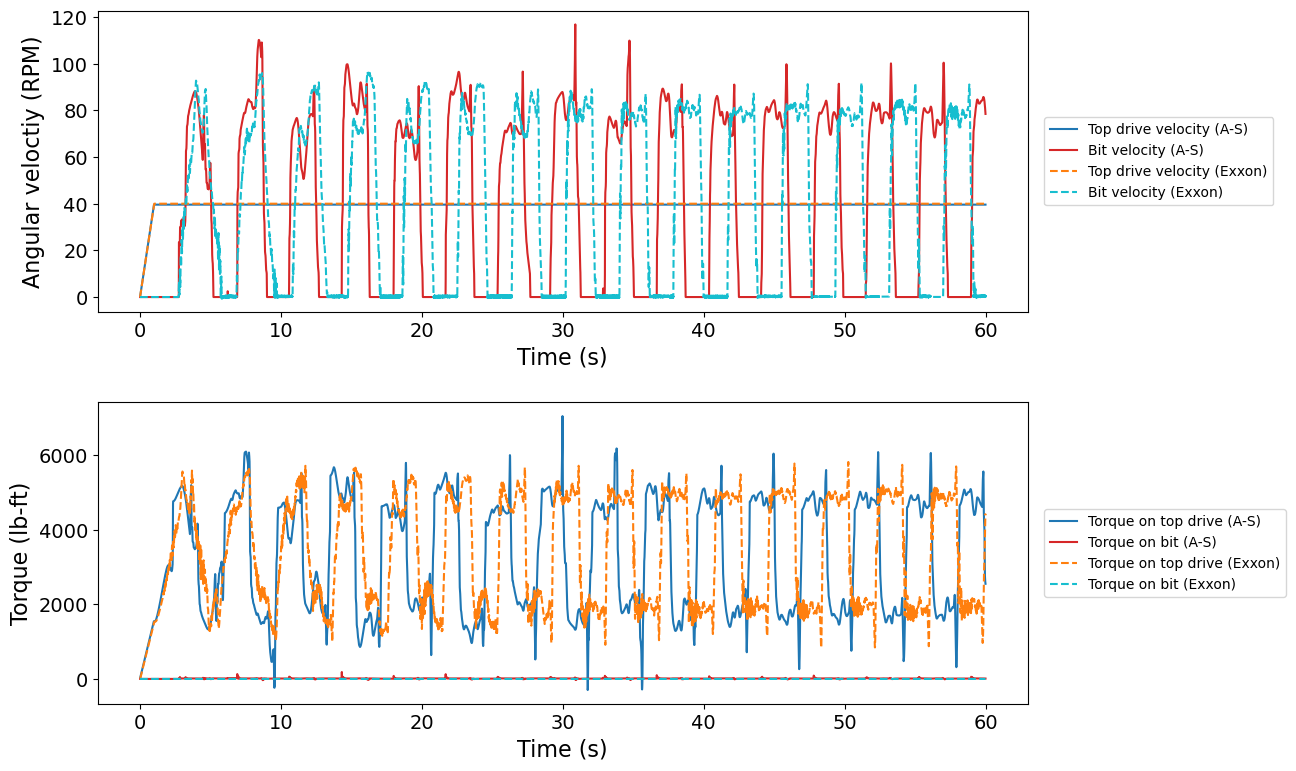
\includegraphics[width=6.5in]{overlapped_figureTestCase4_2}
  \caption{}\label{figure_testcase4_2_overlapped}
\end{figure}
